\documentclass[Thesis.tex]{subfiles}
\begin{document}
\setkeys{Gin}{draft=false}
\chapter{{\sc VaryLab} - Discrete surface optimization}
\label{chp:varylab}

\section{Introduction}

\begin{figure}
    \begin{center}
    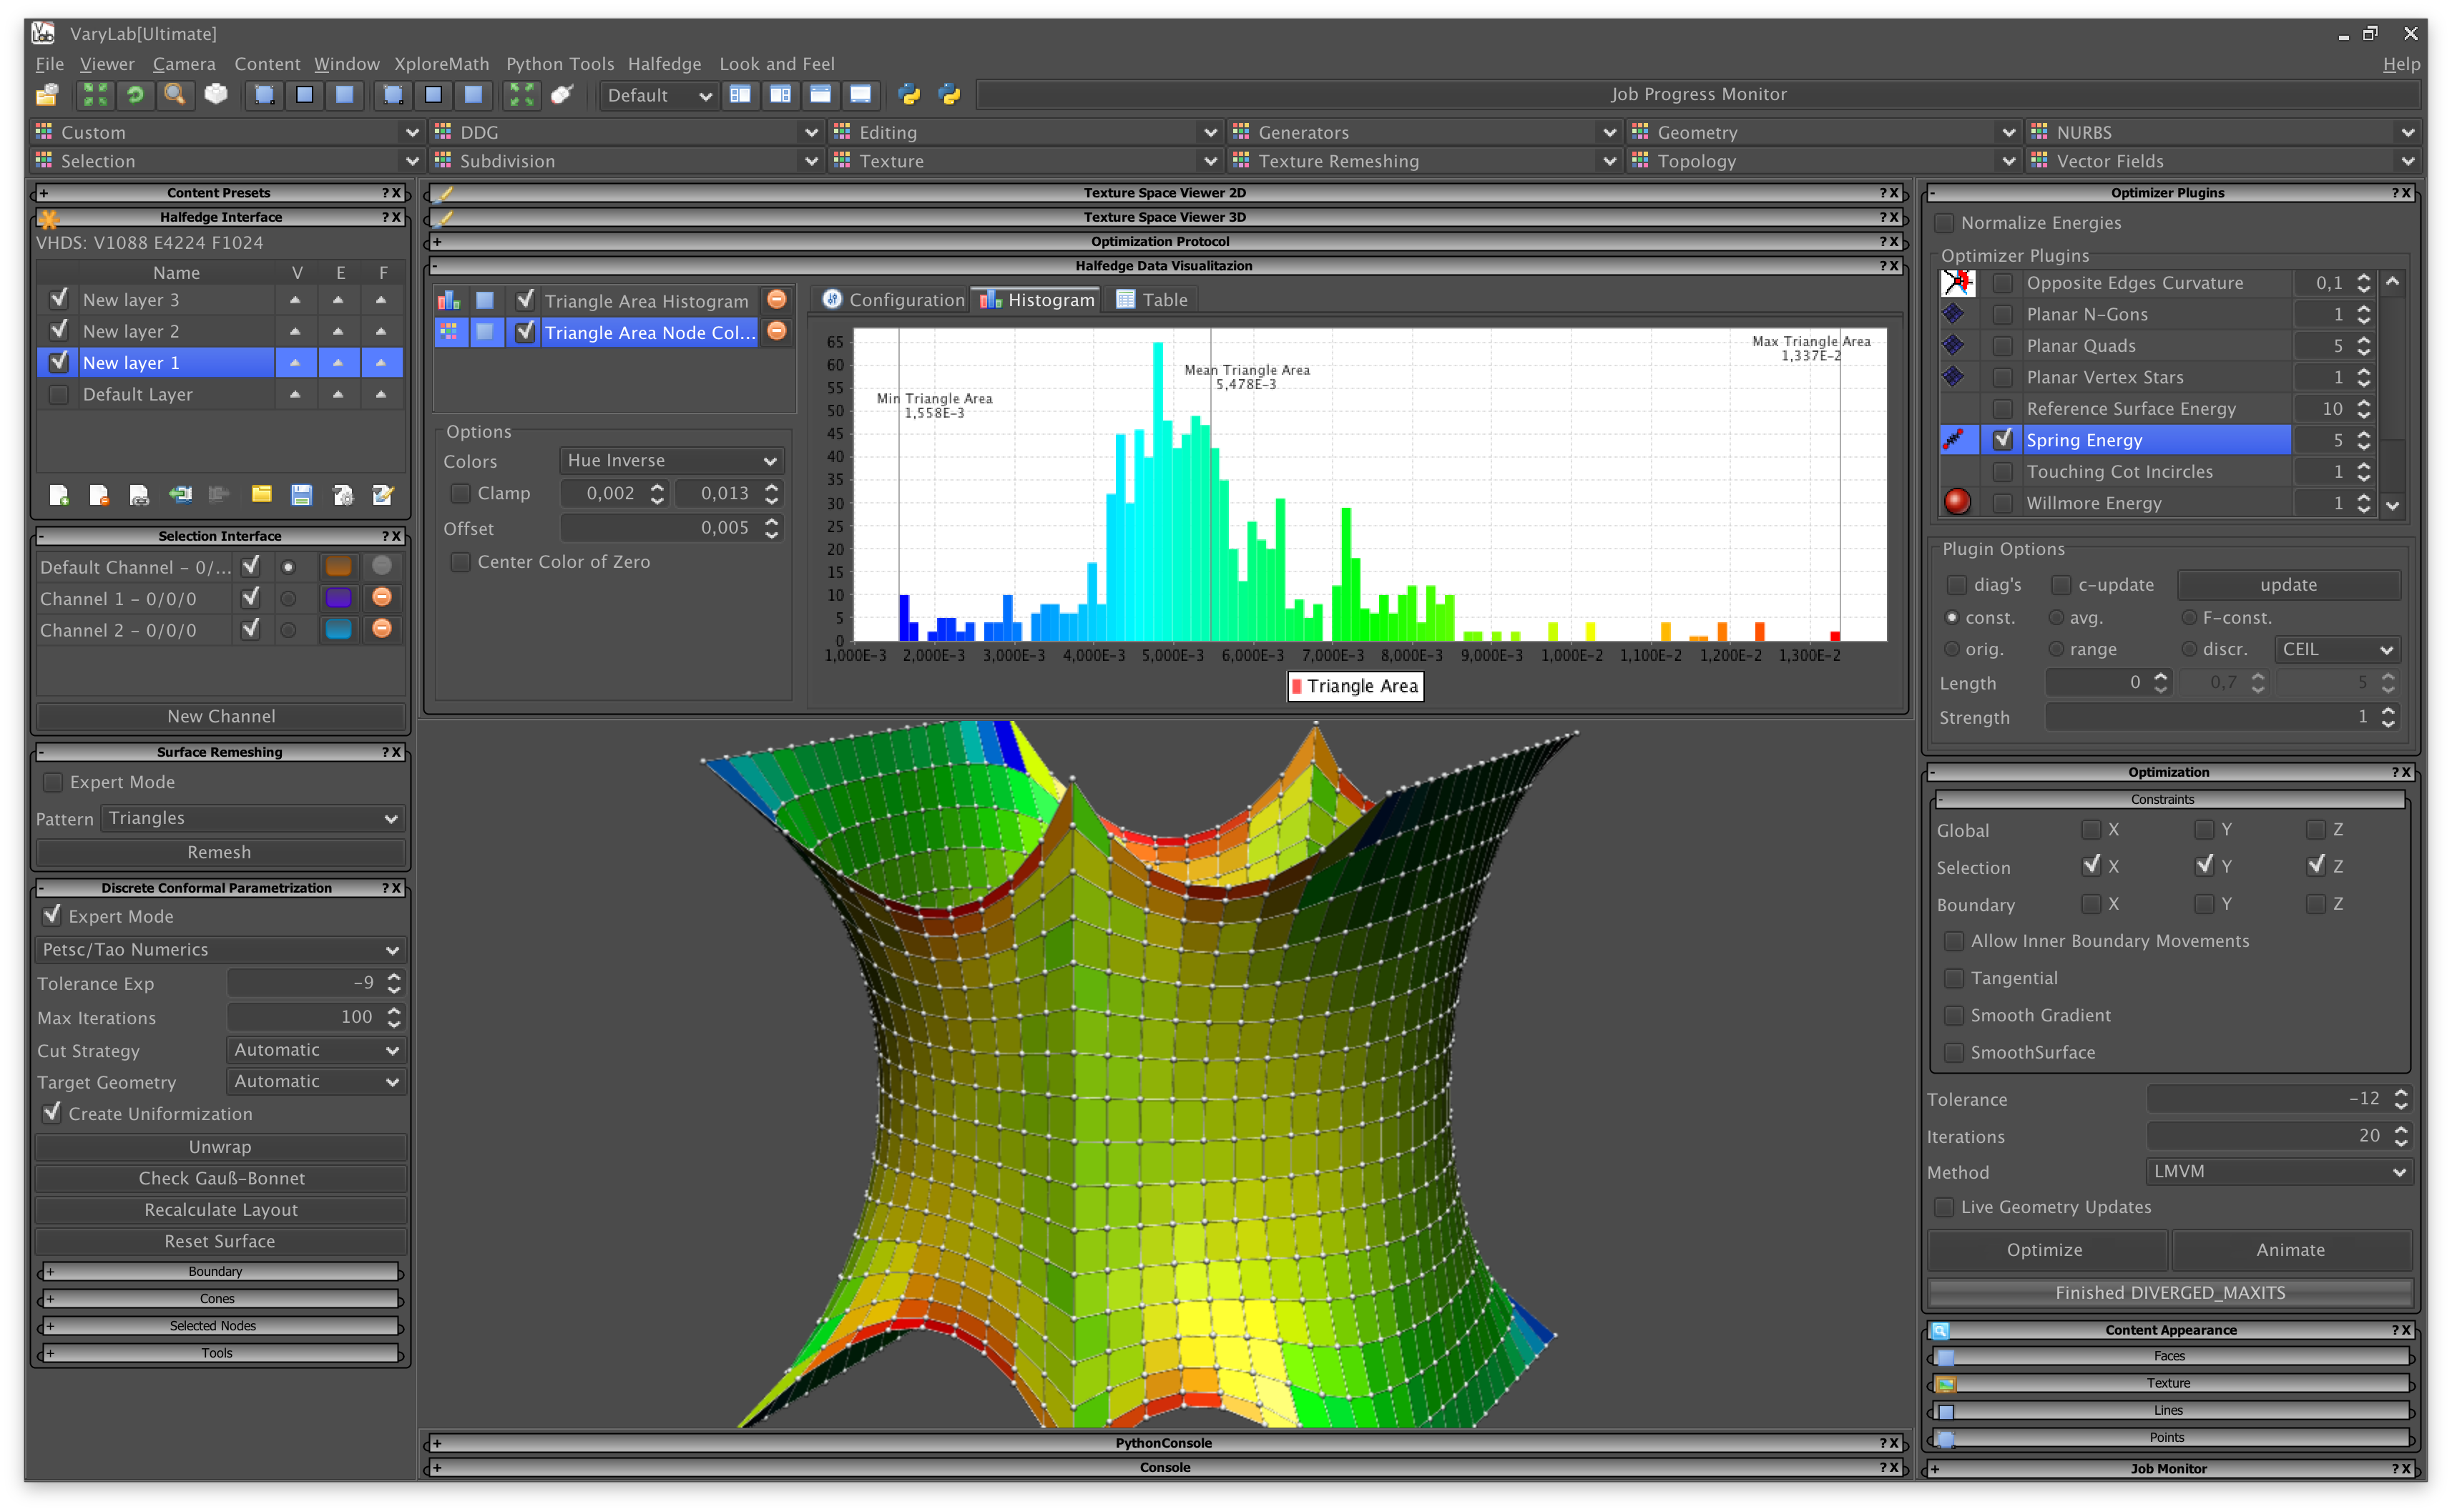
\includegraphics[width=0.8\textwidth]{varylab/varylab_main.png}
    \caption{{\sc VaryLab} main user interface window. Visualization interface (top), energy configuration and optimization tools (right), layers, selections, etc. (left).}
    \label{fig:varylab_main_ui}
    \end{center}
\end{figure}

In this chapter we introduce the {\sc Java} software {\sc VaryLab}. It is a software developed at Berlin Institute of Technology by the author, Thilo R\"orig, and others. It is supported by DFG \mbox{SFB/TRR}~109 Discretization in Geometry and Dynamics. It is designed to be an extensible and modular tool for experiments with discrete surfaces in pure mathematics and applications in industrial geometry. The purpose of this chapter is to enable the reader to reproduce the results presented in Part~\ref{part:applications} of this work.

We start with a general description of {\sc VaryLab} and its features in Section~\ref{sec:general_varylab}. Section~\ref{sec:ui_varylab} introduces the user interface which is based on {\sc JRWorkspace}, see Chapter~\ref{chp:jrworkspace}. Section~\ref{sec:periodic_varylab}, gives details on the use of {\sc VaryLab} when calculating the examples of Chapter~\ref{chp:periodic_conformal_maps}. Section~\ref{sec:quasiisothermic_varylab} explains the steps needed to reproduce results presented in Chapter~ref{chp:quasiisothermic}. Finally, in Section~\ref{sec:gridshells_varylab} we present the capabilities of {\sc VaryLab} when calculating gridshell nets as explained in Chapter~\ref{chp:gridshells}.

In this chapter words in [Brackets] describe ui elements.

\section{Non-linear discrete surface optimization}
\label{sec:general_varylab}
In its core {\sc VaryLab} is a solver for non-linear optimization problems on the coordinates of a given 3D discrete surface. That means given a surface $S$ and functionals $f_1,\ldots,f_n:S\to\R$ we (try to) minimize the combined functional

\begin{eqnarray*}
	f(S) = \sum_{i=1}^n \lambda_i f_i(S)
\end{eqnarray*}
where $\lambda_1,\ldots,\lambda_n\in \R$ are user defined weights. Correspondingly the first and second  derivatives of $f_i(S)$ are weighted by $\lambda_i$
\begin{eqnarray*}
	\nabla f(S) = \sum_{i=1}^n \lambda_i \nabla f_i(S), \quad \nabla\nabla f(S) = \sum_{i=1}^n \lambda_i \nabla\nabla f_i(S).
\end{eqnarray*}

{\sc VaryLab} uses the numerical library {\sc PETSc}/{\sc TAO} \cite{petsc-user-ref, petsc-web-page, tao-user-ref} and the corresponding {\sc Java} bindings \cite{jpetsctao-web-page} for computations. To run optimization methods we need at least an implementation of the functional's value. Other methods need gradient or Hessian of the functional. The most important methods are
 
\begin{tabular}{c | c | c}
	$f$ & $f$, $\nabla f$ & $f$, $\nabla f$, $\nabla\nabla f$\\ \hline
	{\tt NM} Nelder-Mead & {\tt LMVM} Limited-Memory, Variable-Metric & {\tt NLS} Newton Line-Search \\
	& {\tt CG} Conjugate Gradient & {\tt NTR} Newton Trust-Region.
\end{tabular}

In {\sc VaryLab} a functional can choose to implement just the value, see Section~\ref{sec:plugin-api}. Additionally it can implement the gradient and the Hessian of $S$. In principle all methods can be used with all functionals even if those do not implement all data needed for the algorithm. {\sc VaryLab} approximates the values of the gradient or the Hessian if they are missing.

\section{Geometry Processing}

The geometry processing core of {\sc VaryLab} is based on {\sc HalfEdge} and {\sc HalfEdgeTools} (Chapter~\ref{chp:halfedge}), i.e., all geometry processing is done with the help of the half-edge data structure and algorithms that run on top of it. Frequently used geometry processing features include

\begin{figure}
    \begin{center}
    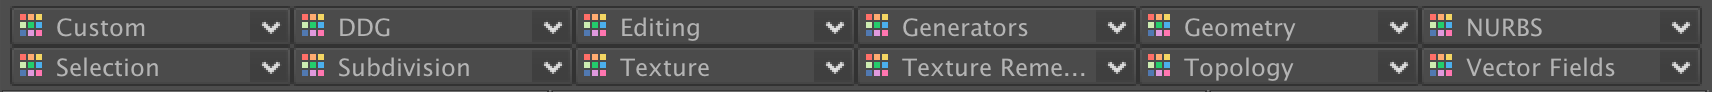
\includegraphics[width=\textwidth]{varylab/tools.png}
    \caption{{\sc VaryLab} tools tool bar.}
    \label{fig:varylab_tools_ui}
    \end{center}
\end{figure}

\begin{itemize}
\item Mesh Generators - Regular Planar Meshes, Convex Hull, Primitive Meshes such as cube, cylinder, sphere, etc.
\item Mesh Editing - Vertex/Edge/Face operations based on user selection.
\item Subdivision - CatmullClark, Doo Sabin, Loop, Sqrt3, etc.
\item Remeshing - Quadritalerals, Triangles, Singularties.
\end{itemize}

All tools are available via the tools tool bar at the top of the main window, see Figure~\ref{fig:varylab_main_ui} and~\ref{fig:varylab_tools_ui}.

\section{Data Visualization}

{\sc VaryLab} adds data sources corresponding to the energies of the optimization core. Their data can be visualized on the surface using the [Halfedge Data Visualization] interface, see Section~\ref{sec:halfedge_tools_visualization}. 

\begin{figure}
    \begin{center}
    \resizebox{\textwidth}{!}{
        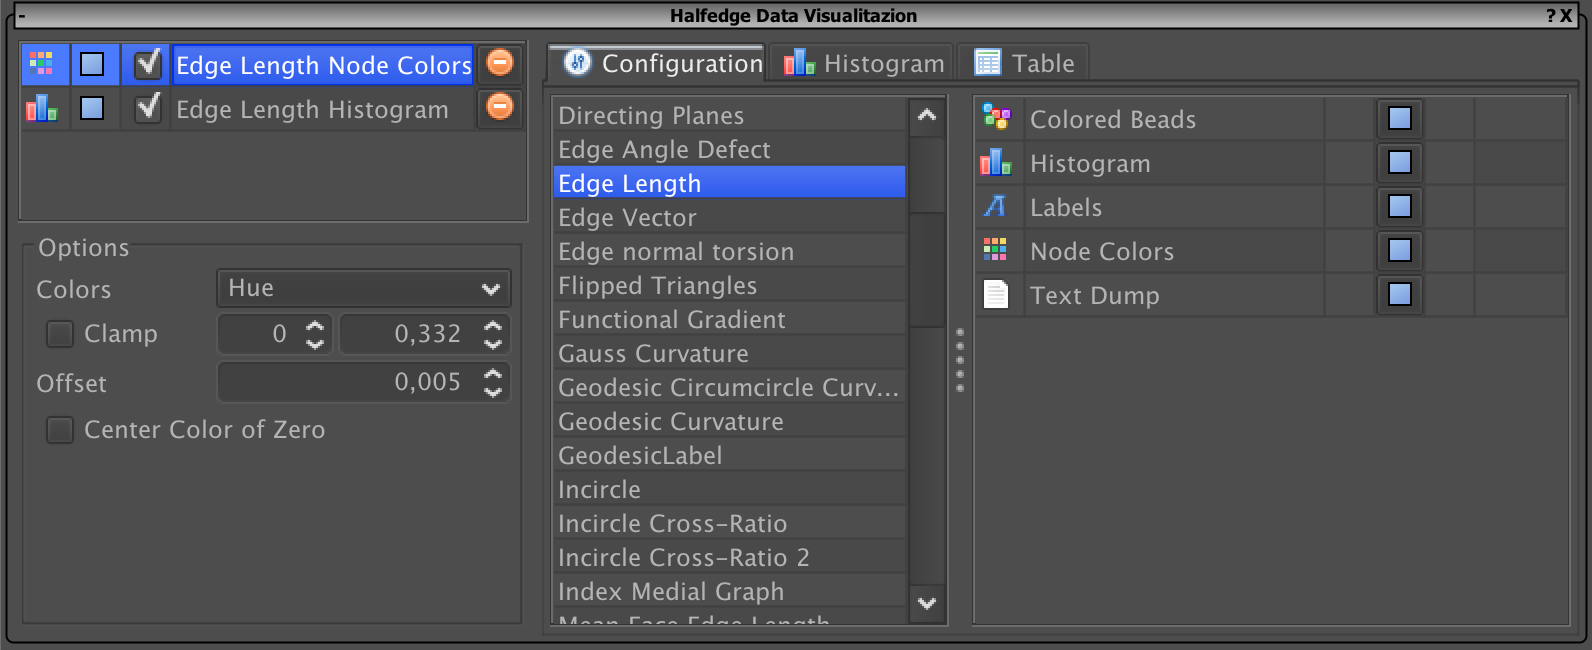
\includegraphics[width=\textwidth]{varylab/edge_visualization.png}
        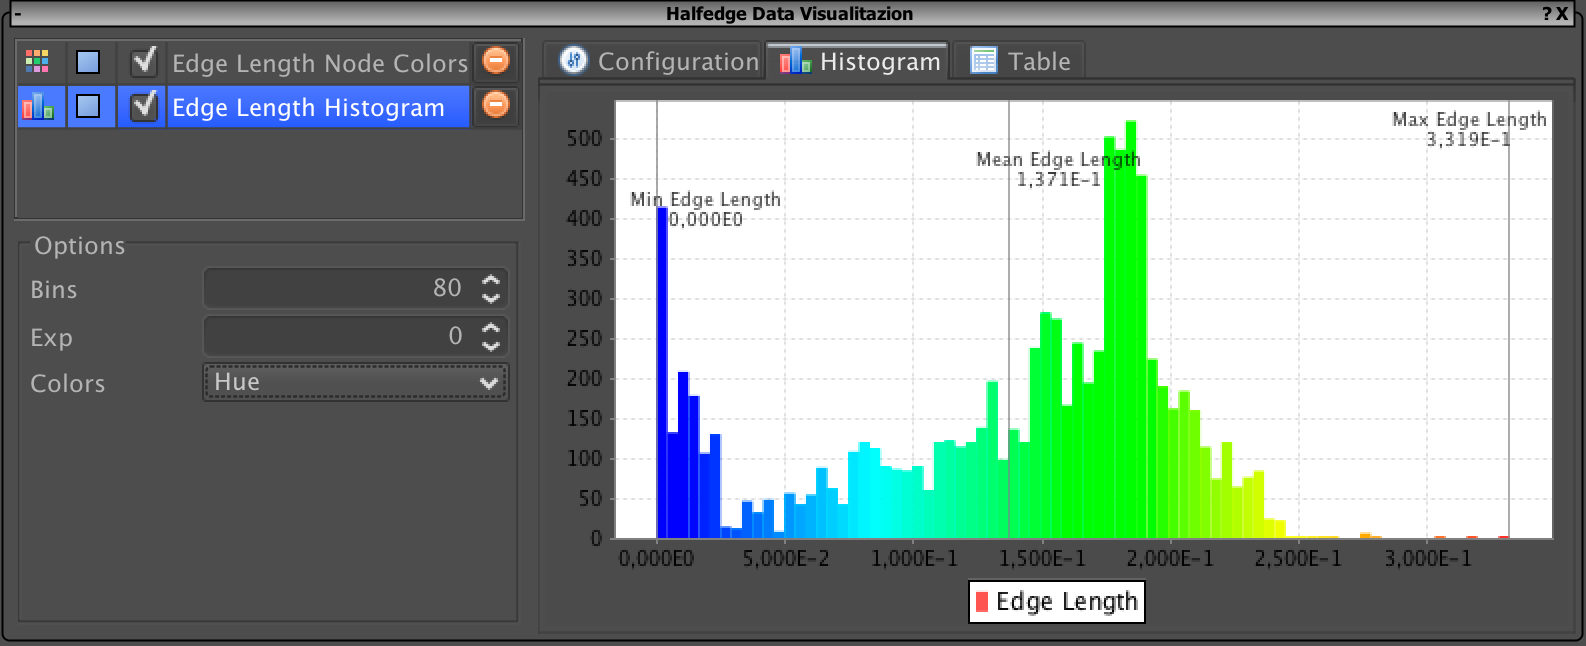
\includegraphics[width=\textwidth]{varylab/edge_histogram.png}    
    }
    \caption{Visualization interface (left), Visualizing mesh edge length data as node colors on a surface and as histogram (right).}
    \label{fig:visualizing_edge_lengths}
    \end{center}
\end{figure}

\begin{example}[Analyzing edge length density] Load some mesh geometry. In the [Halfedge Data Visualization] select the [Edge Length] data source. It provides scalar data for edges of the mesh. Select the [Histogram] and [Node Colors] visualizers to create colored edges and a corresponding histogram for the edge lengths of the mesh, see Figure~\ref{fig:visualizing_edge_lengths}.
\end{example}

\setkeys{Gin}{draft=true}

%Derivatives and numerical substitutes, 
%Boundary Conditions
%Numerics
%Build-In Functionals
%Plug-in facility and extensibility, 
%Data Visualization (scalar, vector)
%Remeshing

\section{User interface}
\label{sec:ui_varylab}

The user interface of {\sc VaryLab}, see Figure~\ref{fig:varylab_main_ui}, is based on {\sc JRWorkspace}, Chapter~\ref{chp:jrworkspace}. Thus it inherits the ability for the user to freely move around all interface components of the main window, see Figure~\ref{fig:varylab_main_ui}. 
The most important interface components are shown in Figure~\ref{fig:optimization_interface_varylab} and \ref{fig:protocol_interface_varylab}.

\begin{figure}
\begin{center}
    \resizebox{\linewidth}{!}{
        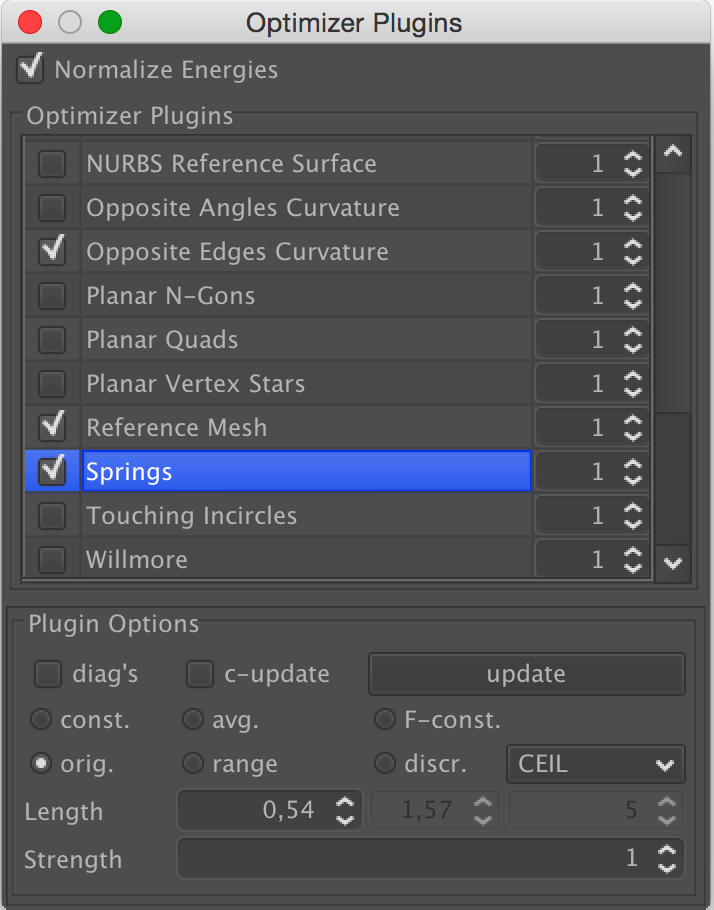
\includegraphics[width=\textwidth]{varylab/optimization_plugins2.png}
        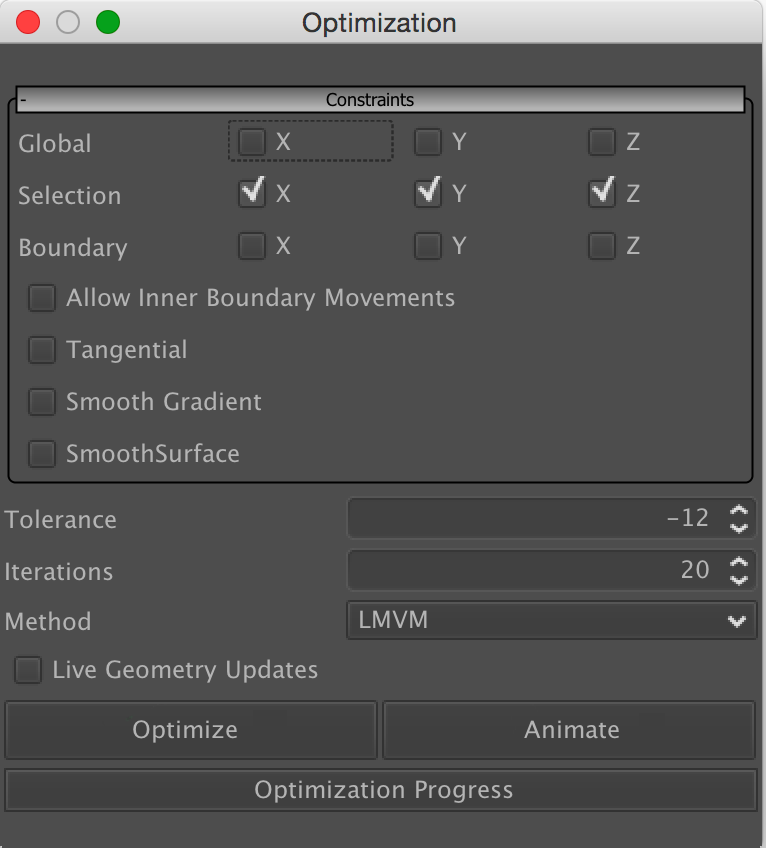
\includegraphics[width=\linewidth]{varylab/optimization2.png}
    }
\caption{The main user interface panels of {\sc VaryLab}. List of optimization functional plug-ins and their options (left). Main optimization controls with global constraints and minimizer settings (right).}
\label{fig:optimization_interface_varylab}
\end{center}
\end{figure}

\begin{figure}
\begin{center}
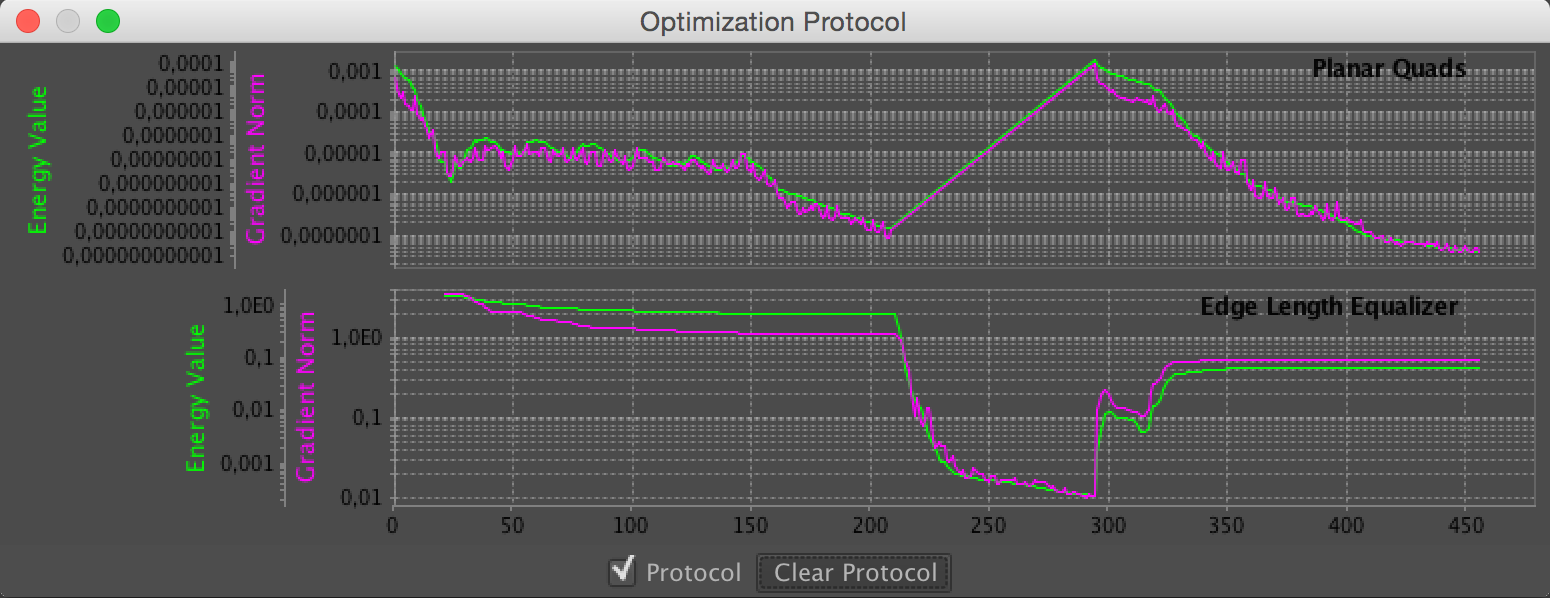
\includegraphics[width=\textwidth]{varylab/protocol.png}
\caption{Optimization protocol panel (bottom) shows the progress of the optimization for each activated energy in the Optimizer Plug-ins panel.}
\label{fig:protocol_interface_varylab}
\end{center}
\end{figure}

\setkeys{Gin}{draft=true}

\section{Periodic conformal maps with {\sc VaryLab}}
\label{sec:periodic_varylab}
In this section we describe how the methods of Chapter~\ref{chp:periodic_conformal_maps} are implemented in {\sc VaryLab}. We split the process in two parts. Part one describes the creation of periodic triangle, quad, or hexagonal meshes from an initial unstructured triangle mesh. Part two deals with optimization of panels created from a mesh in part one.

\subsection{Periodic Parameterization}
The parameterization part of the work is carried out via the {\sc ConformalLab} main user interface. 

\begin{itemize}
\item[0] Load a surface with two boundary components. You can map the surface using the three methods described in the article, map to a cylinder (a), polygonal map to a cone of revolution (b), and isometric boundary (c) to an adapted cone of revolution.
\item[1(a)] For the map to the cylinder create a conformal parameterization with straight boundary using the [Discrete Conformal Parameterization] panel and [Quantized Angles/Straight] boundary mode. A cut is introduced automatically to uniquely define the map.\\

\begin{center}
\begin{minipage}{0.9\linewidth}
            \centering
            \resizebox{\linewidth}{!}{
            	\includegraphics{periodic/step00.png}
            	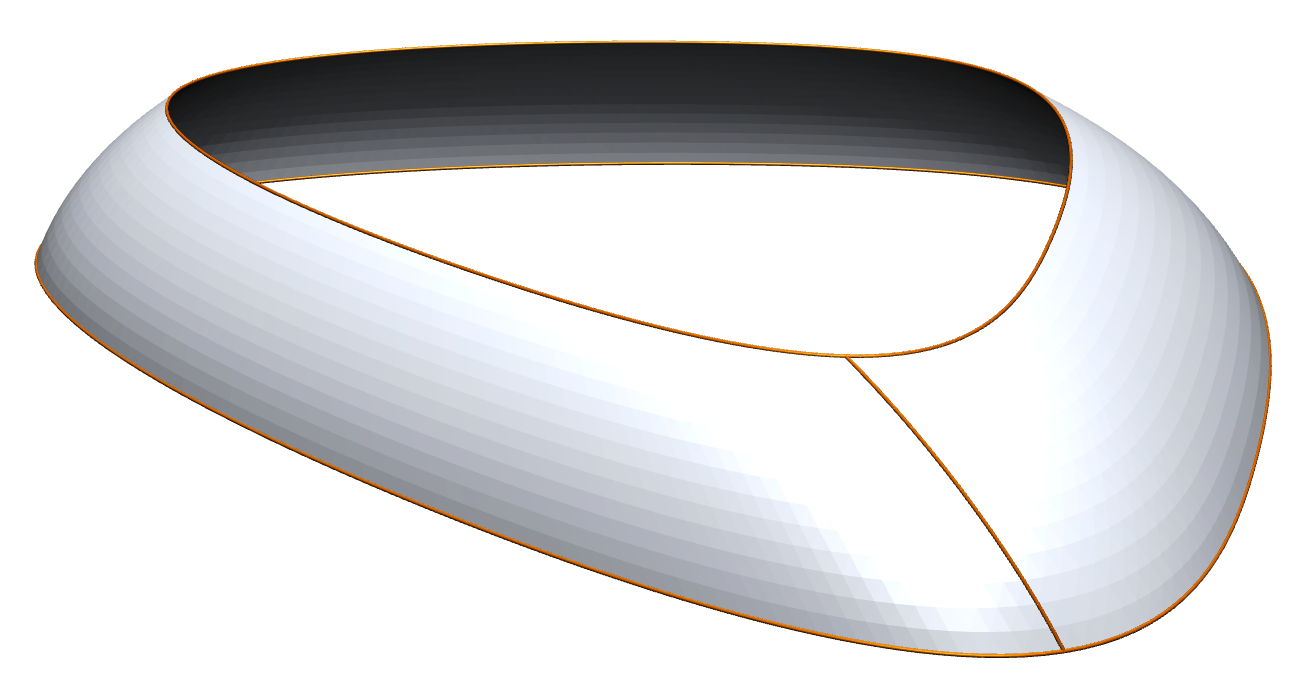
\includegraphics{periodic/step01_surface.png}	
            	\includegraphics{periodic/step02_surface.png}		
            }
            \resizebox{\linewidth}{!}{
                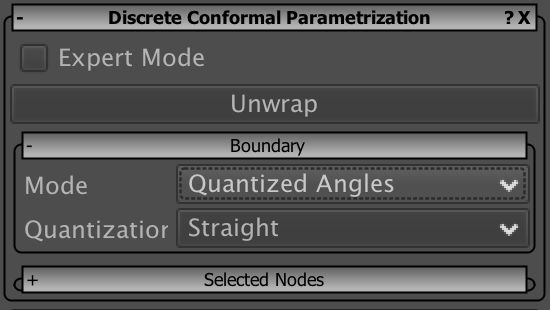
\includegraphics[width=3.2cm]{periodic/step01_ui.png}
                \begin{minipage}[b]{10cm}
                    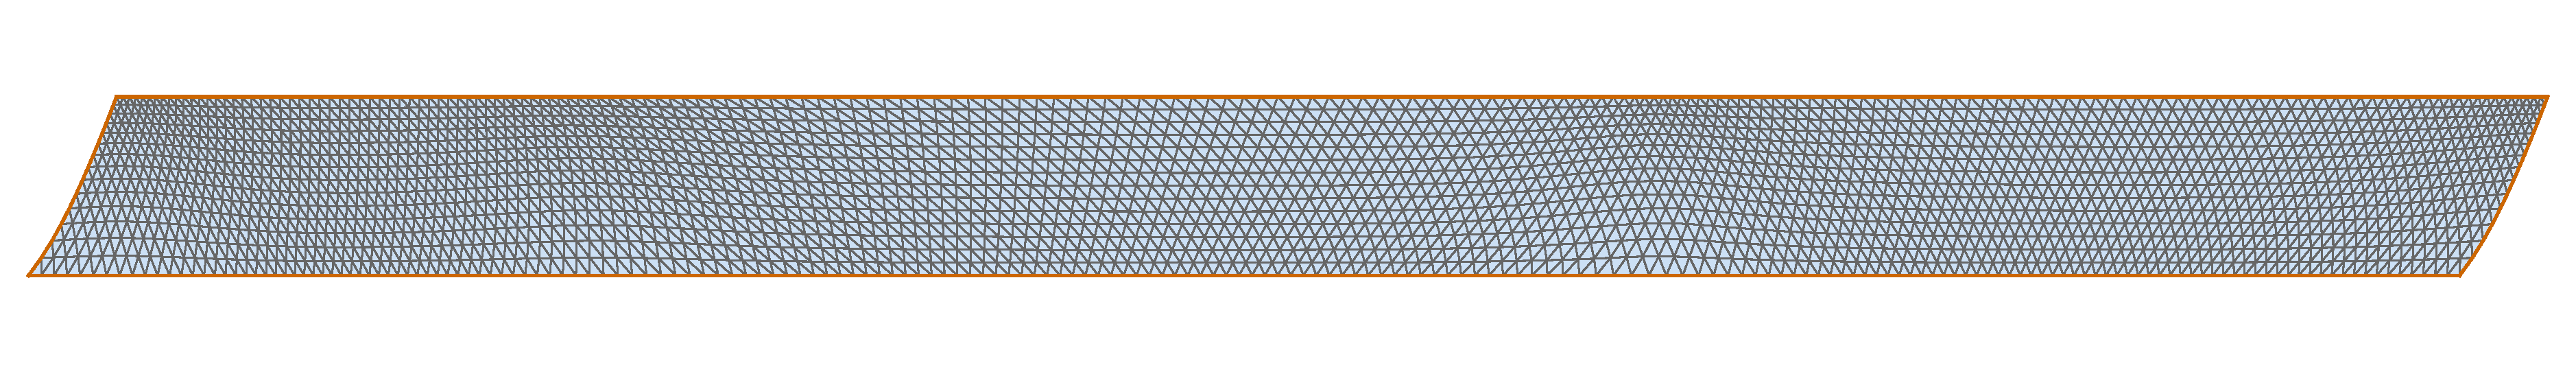
\includegraphics[width=\linewidth]{periodic/step01a_map.pdf}\\
                    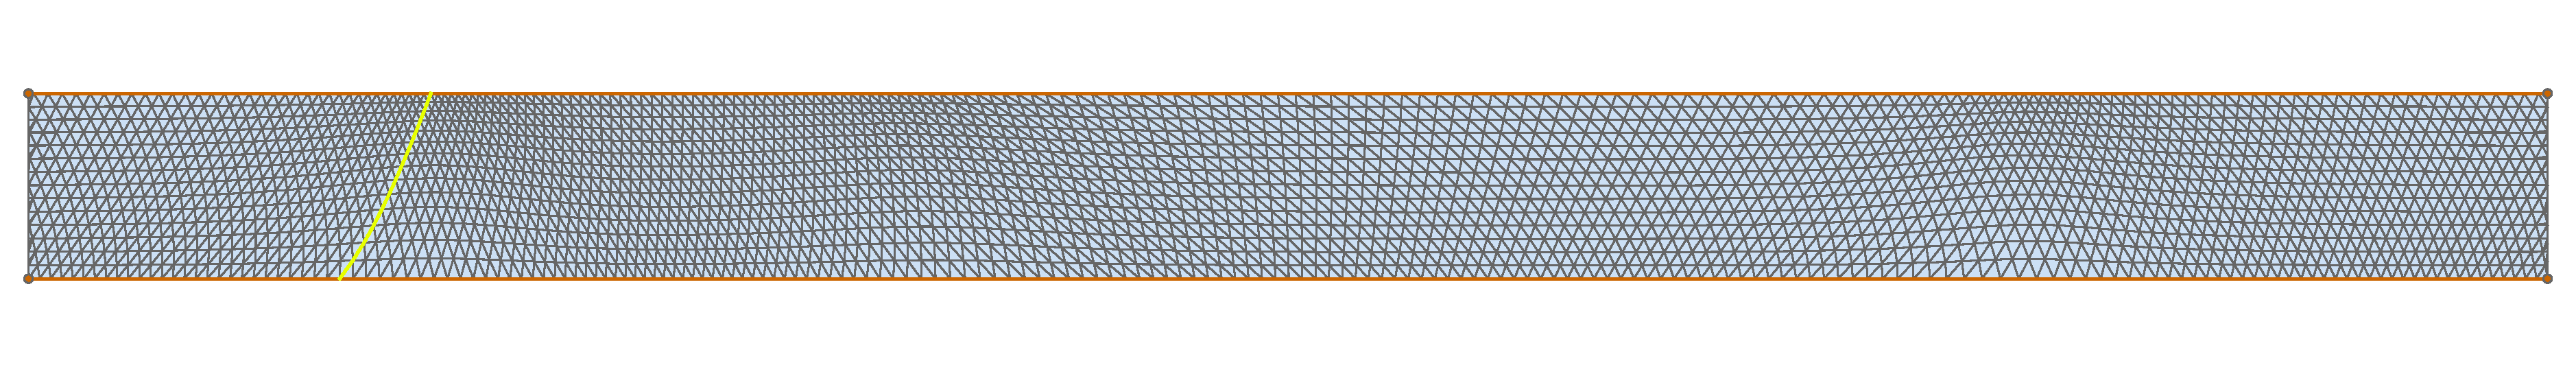
\includegraphics[width=\linewidth]{periodic/step02a_map.pdf}
                \end{minipage}
            }
            \captionof{figure}{Map to cylinder. Start with an automatically cut mesh (top-middle and upper domain image) and modify the cut (top-right and lower domain image) such that the remeshing algorithm can handle the complete boundary.}
            \label{fig:periodic_algorithm1a}
\end{minipage}
\end{center}            

\item[1(b)] For a polygonal map to a cone of revolution, select boundary vertices to specify boundary angles for the domain. Use multiples of $\frac{\pi}{3}$ for triangle/hexagonal panels and multiples of $\frac{\pi}{4}$ for quadrilaterals.

\begin{center}
\begin{minipage}{0.9\linewidth}
            \centering
            \resizebox{0.7\textwidth}{!}{
            	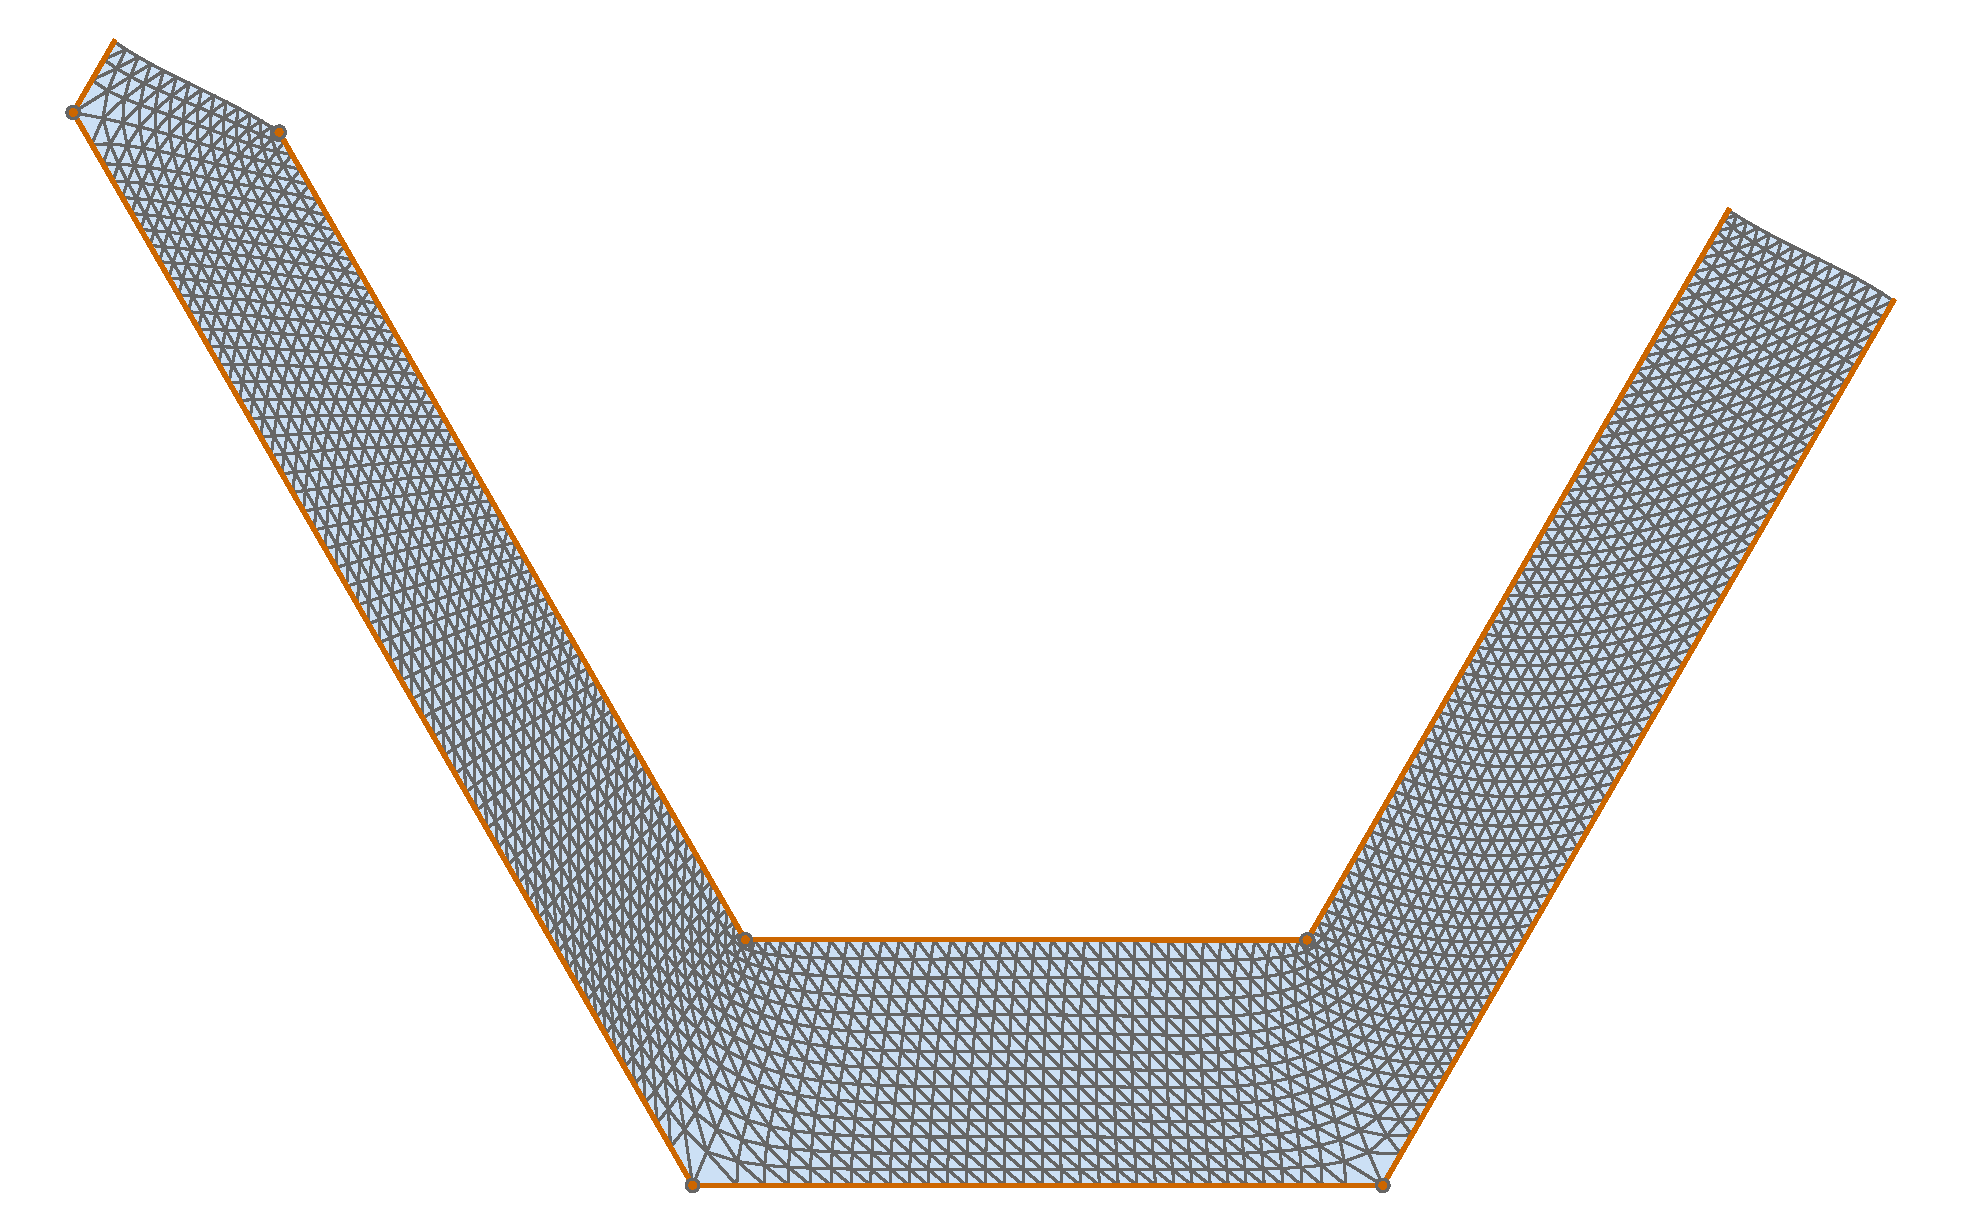
\includegraphics{periodic/step01b_map.pdf}
            	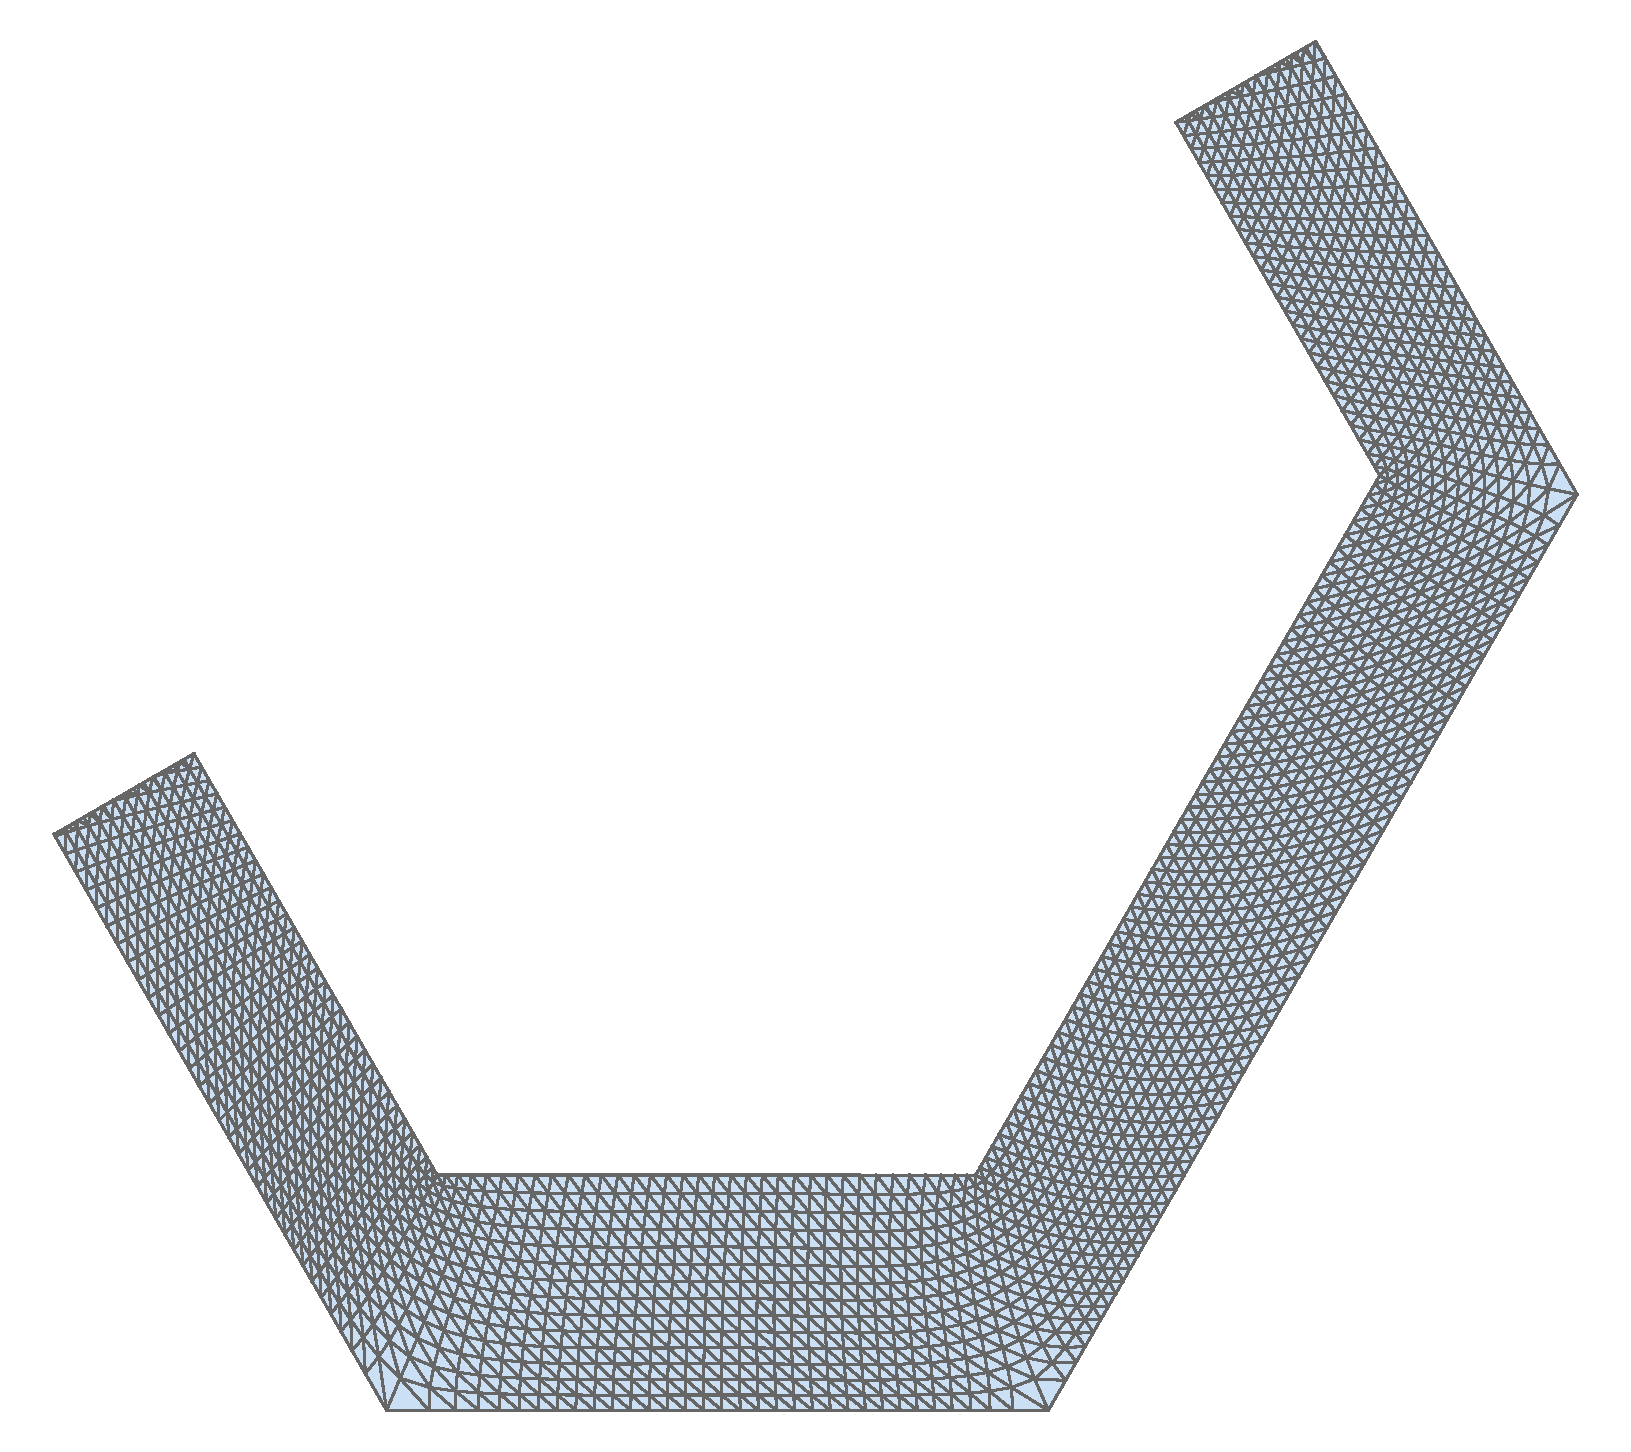
\includegraphics{periodic/step02b_map.pdf}	
            }
            \captionof{figure}{Mapping the surface from Figure~\ref{fig:periodic_algorithm1a} to a hex pattern adapted domain with polygonal boundary curve. Cut orthogonal to the boundary to create a domain that can easily be meshed with boundary aligned hexagons. The domain is identified along the cut via a rotation by $\pi$.}
\end{minipage}
\end{center}

\item[1(c)] Create an isometric boundary and a map to cone of revolution using the [Read Isometric Angles] boundary mode and the [NoCuts] cut strategy. It creates a map to an arbitrary cone of revolution and reads off the resulting boundary angles. Those are set as new boundary conditions (red vertex selection). In a second step choose the [Quantized Angle Periods] boundary mode and the desired quantization for the final map to the pattern adapted cone of revolution.

\begin{center}
\begin{minipage}{0.9\linewidth}
            \centering
            \resizebox{\linewidth}{!}{
            	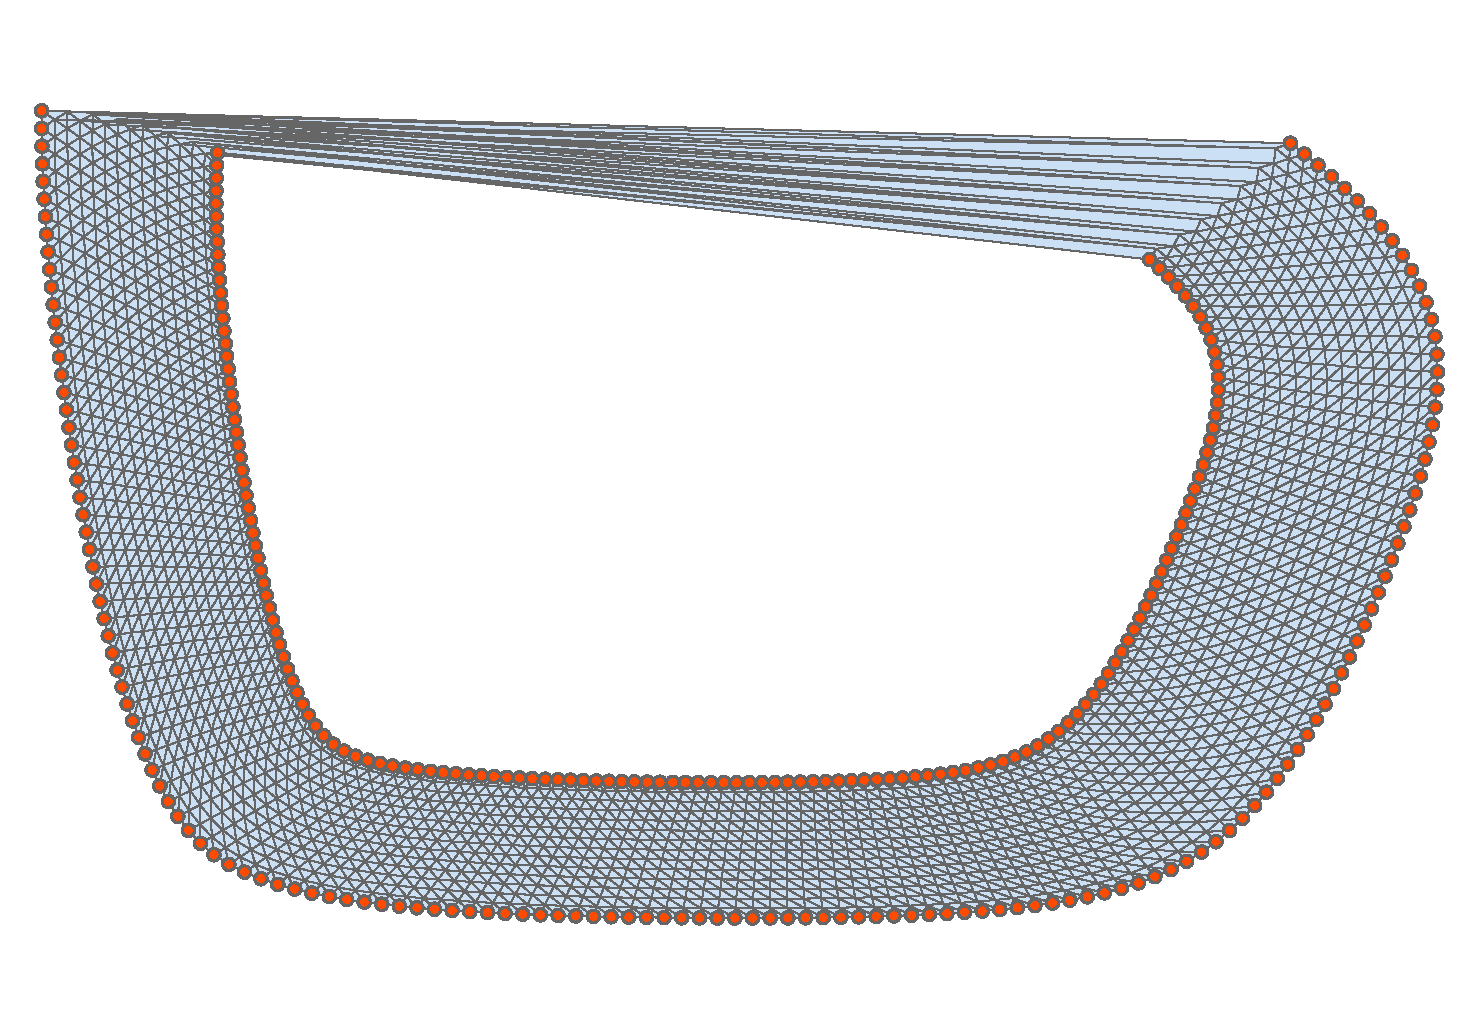
\includegraphics[width=5cm]{periodic/step01c_map.pdf}
            	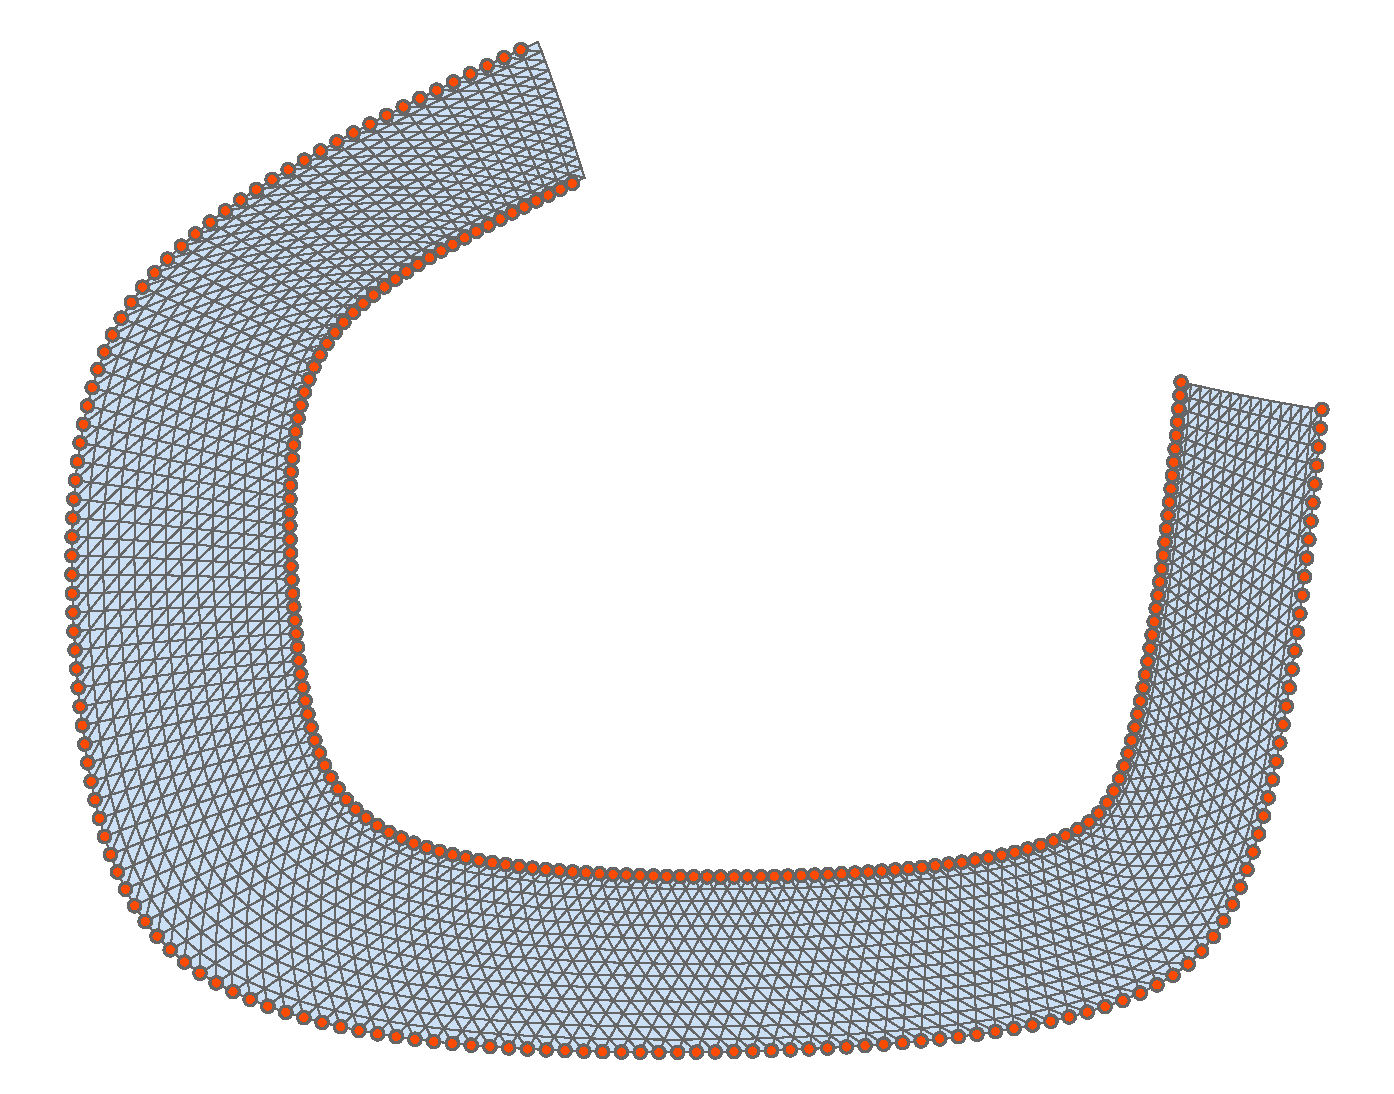
\includegraphics[width=5cm]{periodic/step02c_map_hexadapted.pdf}	
            	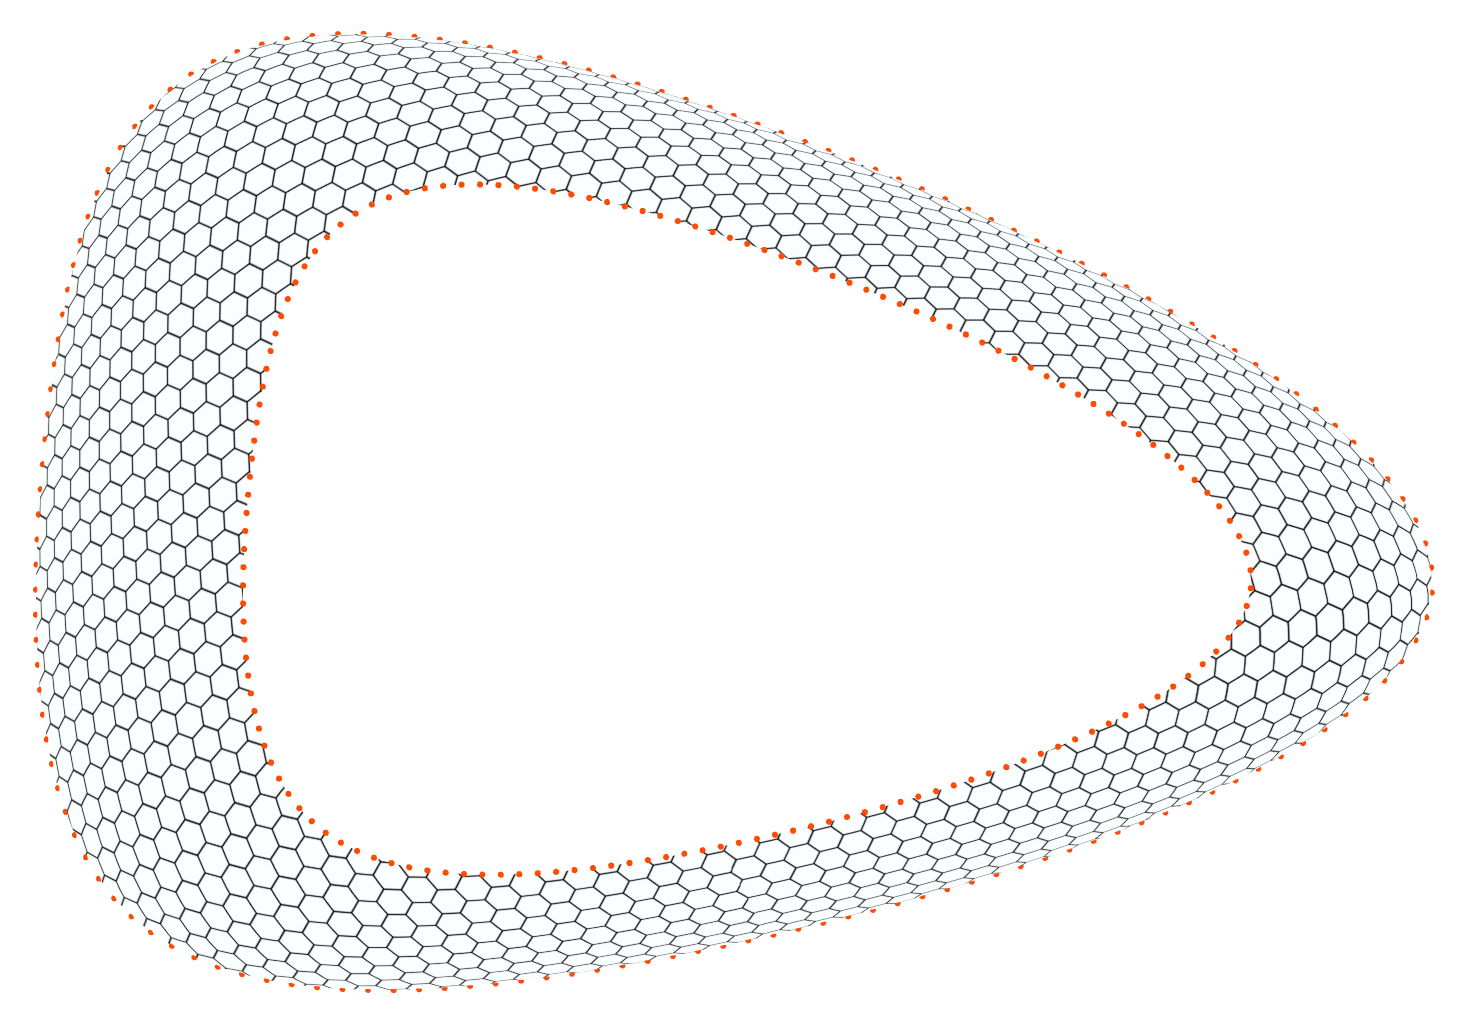
\includegraphics[width=6cm]{periodic/step02c_surface.png}		
            }
            \captionof{figure}{Map to cylinder with isometric boundary. Create a map with isometric boundary without cutting the mesh (left). Modify the resulting boundary angles to support a periodic pattern (middle). Periodic hexagonal pattern on the surface (right)}
\end{minipage}
\end{center}    

\item[2] Use the [Cut and Glue Texture Domain] command and select [Orthogonal to Boundary] to create a map to a rectangle (a), a map to a polygonal region (b). In the isometric boundary case (c) we do not need a polygon as boundary curve.
\item[3] Select a predefined texture for quadrilateral, triangle, or hexagonal mesh preview from the [Content Appearance$\to$Texture] panel. Adjust the texture scale to a reasonable value. In the isometric case (c) close the period with the texture transformation user interface manually. For cases (a) and (b) periods will be closed automatically by the remeshing algorithm.

\begin{center}
\begin{minipage}{0.9\linewidth}
            \centering
            \resizebox{\linewidth}{!}{
            	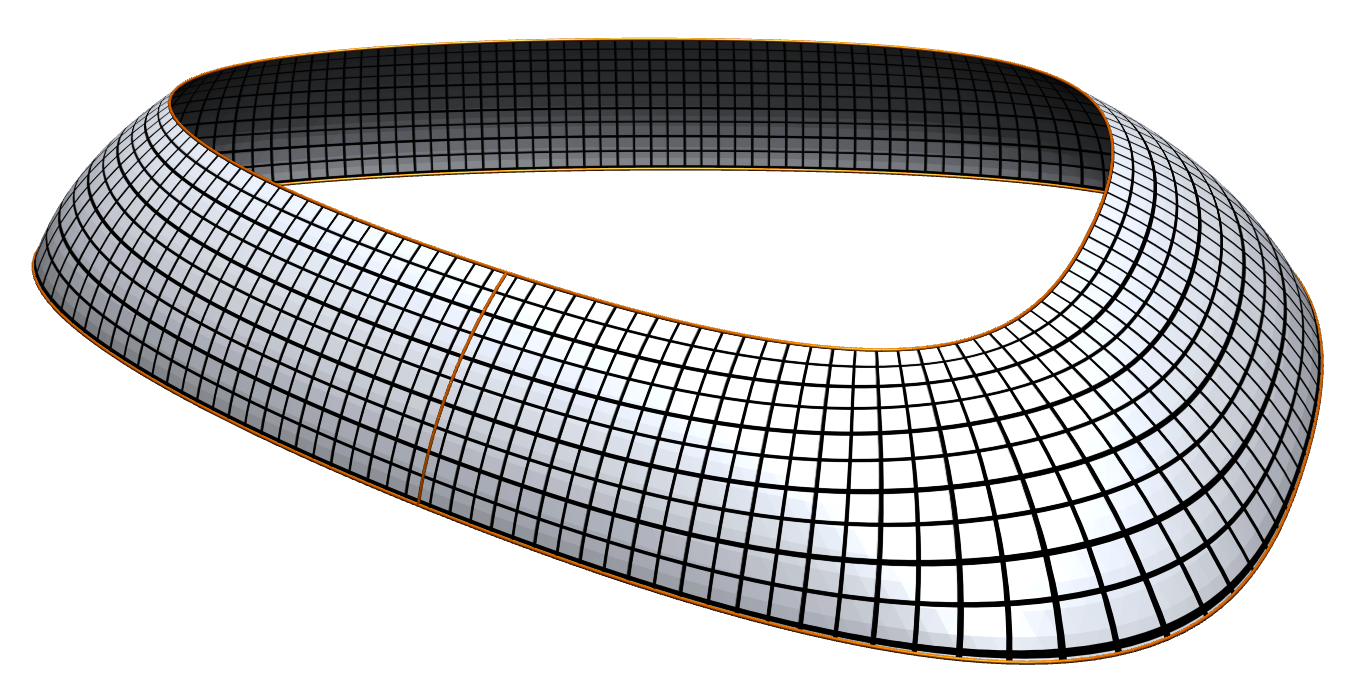
\includegraphics[width=5cm]{periodic/step03_quads.png}
            	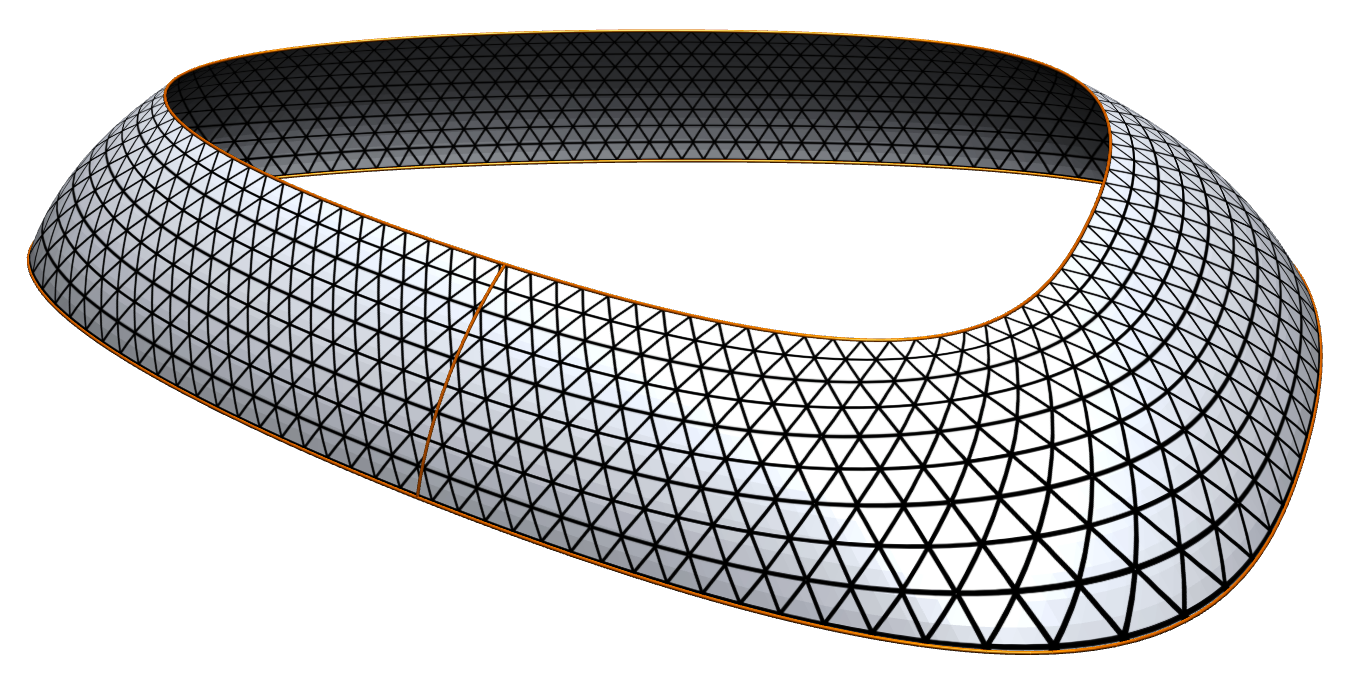
\includegraphics[width=5cm]{periodic/step03_triangles.png}	
            	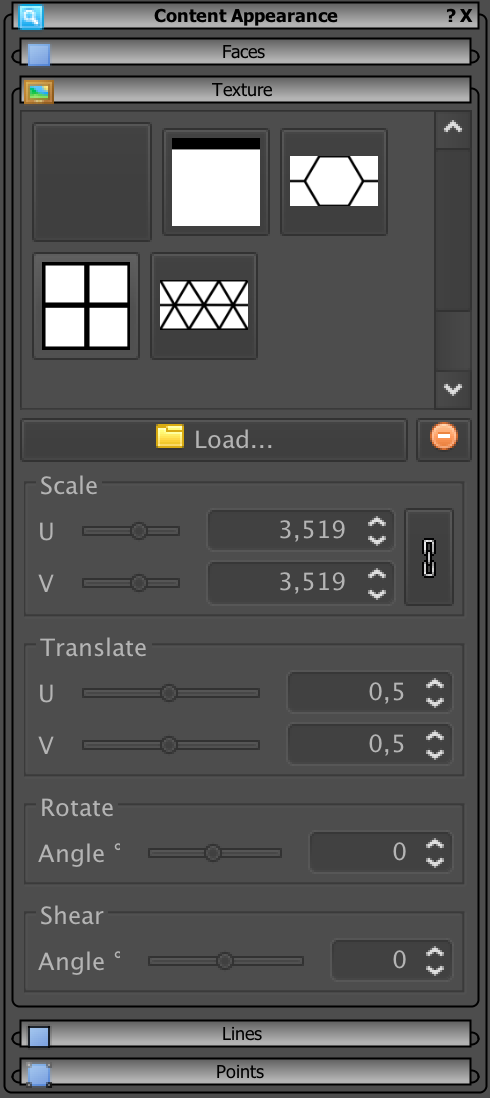
\includegraphics[width=1.5cm]{periodic/step03_ui.png}	
            }
            \captionof{figure}{Pattern preview.}
\end{minipage}
\end{center}    

\item[4] Perform remeshing in cases (a) and (b) either for [Boundary Aligned Triangles] or [Boundary Aligned Quads] using the [Surface Remeshing] panel. For non-boundary aligned parameterization (c) use the [Quads With Singularities/Triangles With Singularities] remeshing mode.\\

\begin{center}
\begin{minipage}{0.9\linewidth}
            \centering
            \resizebox{\linewidth}{!}{
            	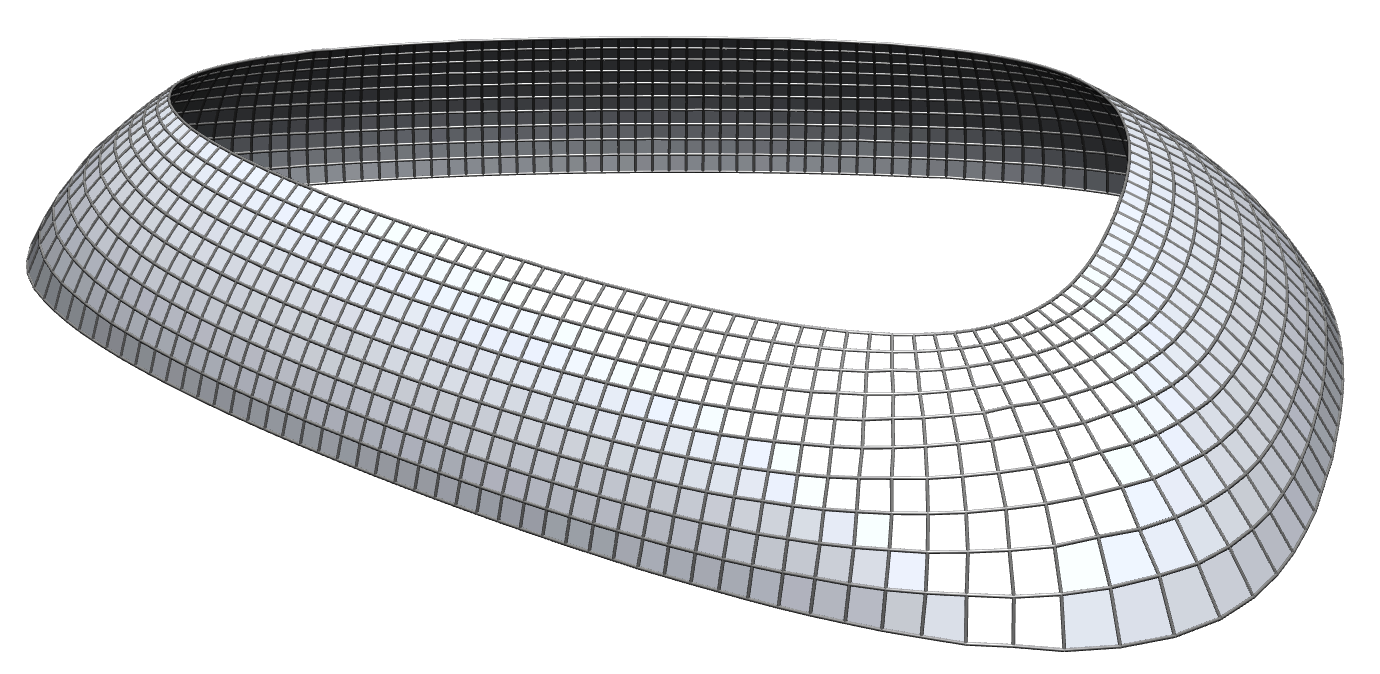
\includegraphics[width=5cm]{periodic/step04_quads_surface.png}
            	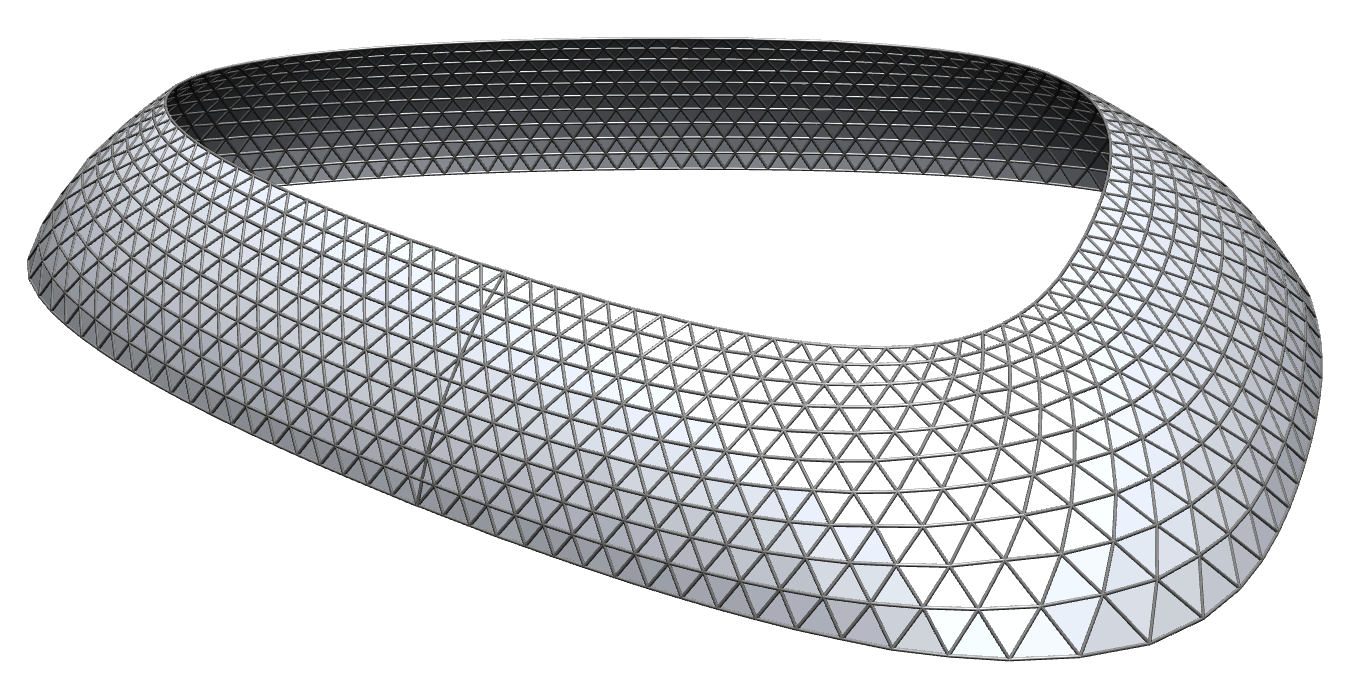
\includegraphics[width=5cm]{periodic/step04_triangles_surface.png}	
            	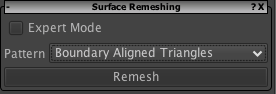
\includegraphics[width=2cm]{periodic/step04_ui.png}	
            }
            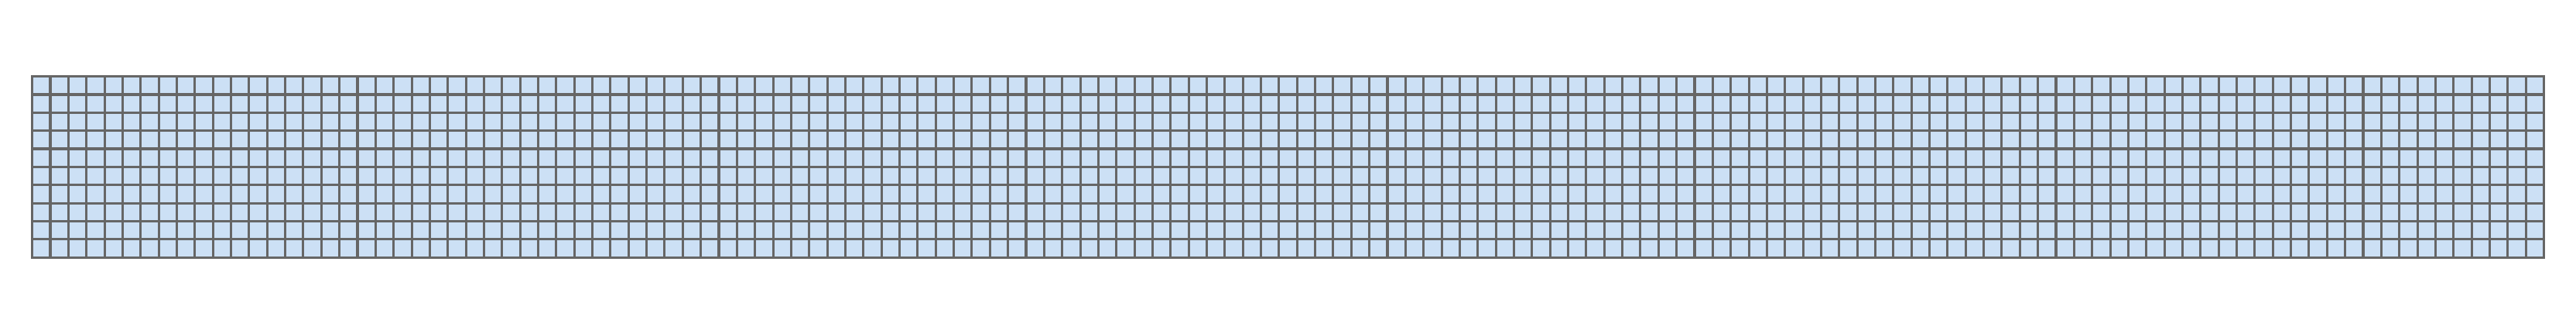
\includegraphics[width=\linewidth]{periodic/step04_quads_map.pdf}
            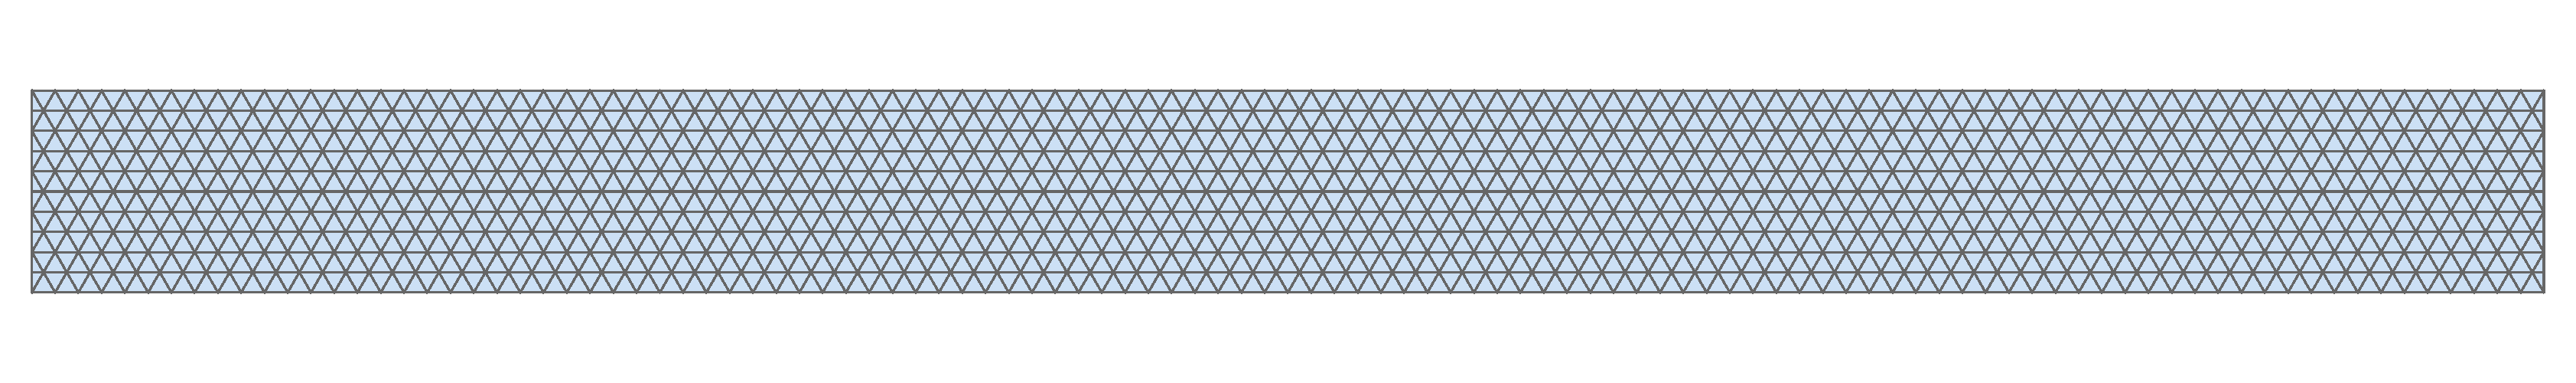
\includegraphics[width=\linewidth]{periodic/step04_triangles_map.pdf}
            \captionof{figure}{New mesh and domain.}
\end{minipage}
\end{center}    

\item[5] Create a watertight mesh using the [Watertight Mesh Generator] and remove extra edges and vertices. In the isometric case (c) use a combination of [Topology$\to$Stitch] and [Topology$\to$Stitch Cut Path] to remove the cut path from the mesh.
\item[6] For hexagonal mesh creation select from the periodic triangle mesh all centers of hexagons using the [Selection$\to$Lattice] command. The [Remove Vertex and Fill] command then creates a periodic hexagonal mesh.
\begin{center}
\begin{minipage}{0.9\linewidth}
            \centering
            \resizebox{\linewidth}{!}{
            	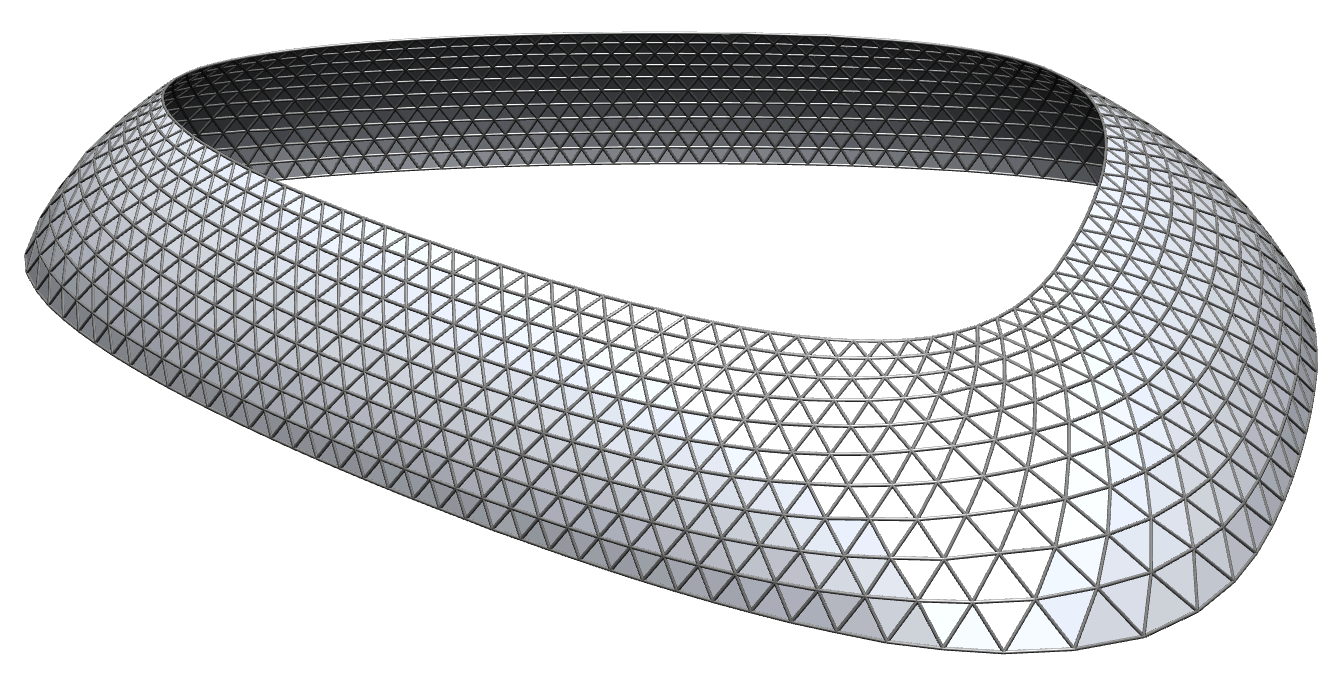
\includegraphics{periodic/step05.png}
            	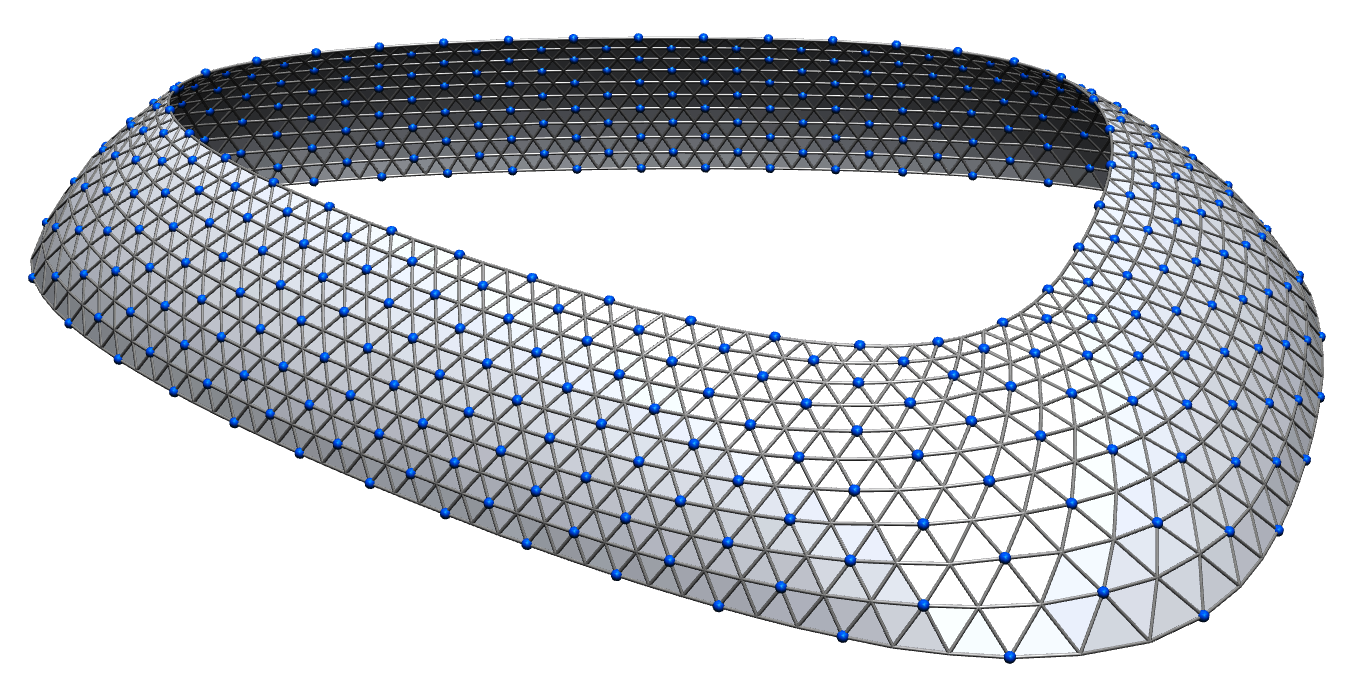
\includegraphics{periodic/step06.png}
            	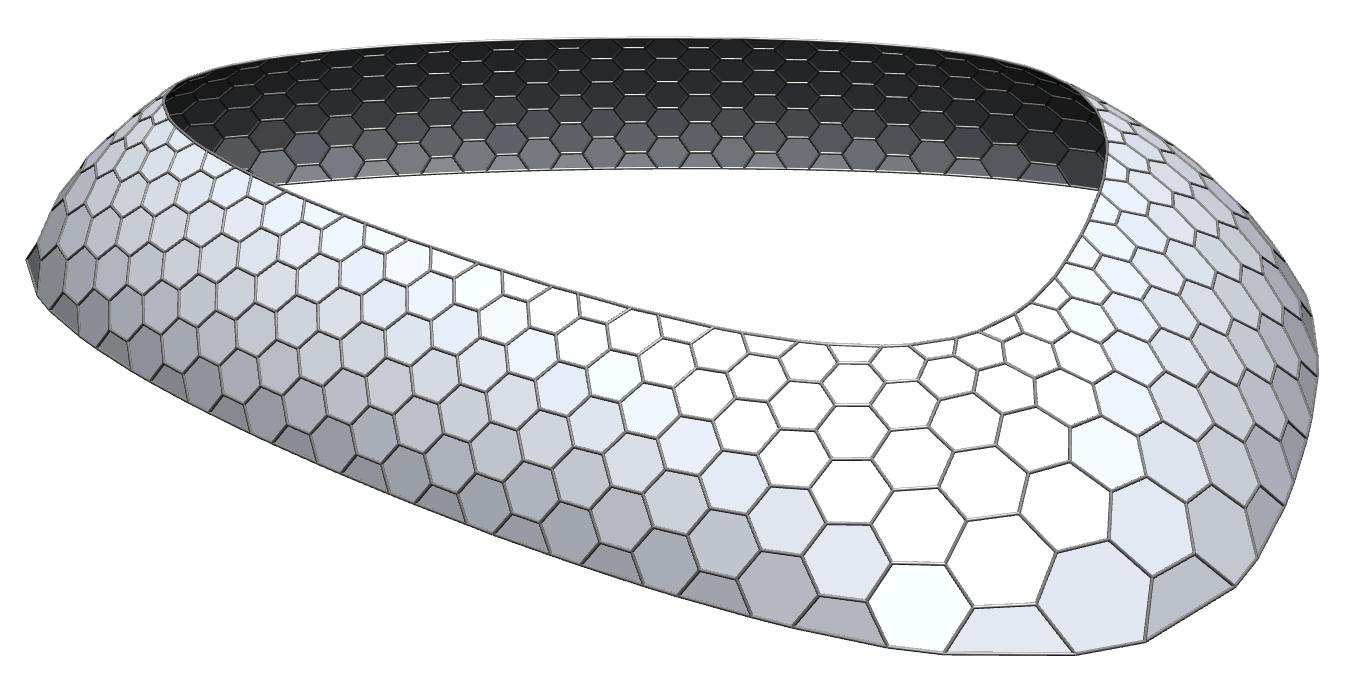
\includegraphics{periodic/step07.png}	
            }
            \captionof{figure}{Creating a periodic hexagonal mesh from a triangle mesh.}
\end{minipage}
\end{center}                
\end{itemize}

\subsection{Panel optimization}

\begin{itemize}
\item[8] [Topology]$\to$[Explode] creates separate faces. Use a [Mean face Edge Length] histogram to show the density of edge lengths. If you want planar panels you should planarize them now.

\begin{center}
\begin{minipage}{0.9\linewidth}
            \centering
            \resizebox{\linewidth}{!}{
            	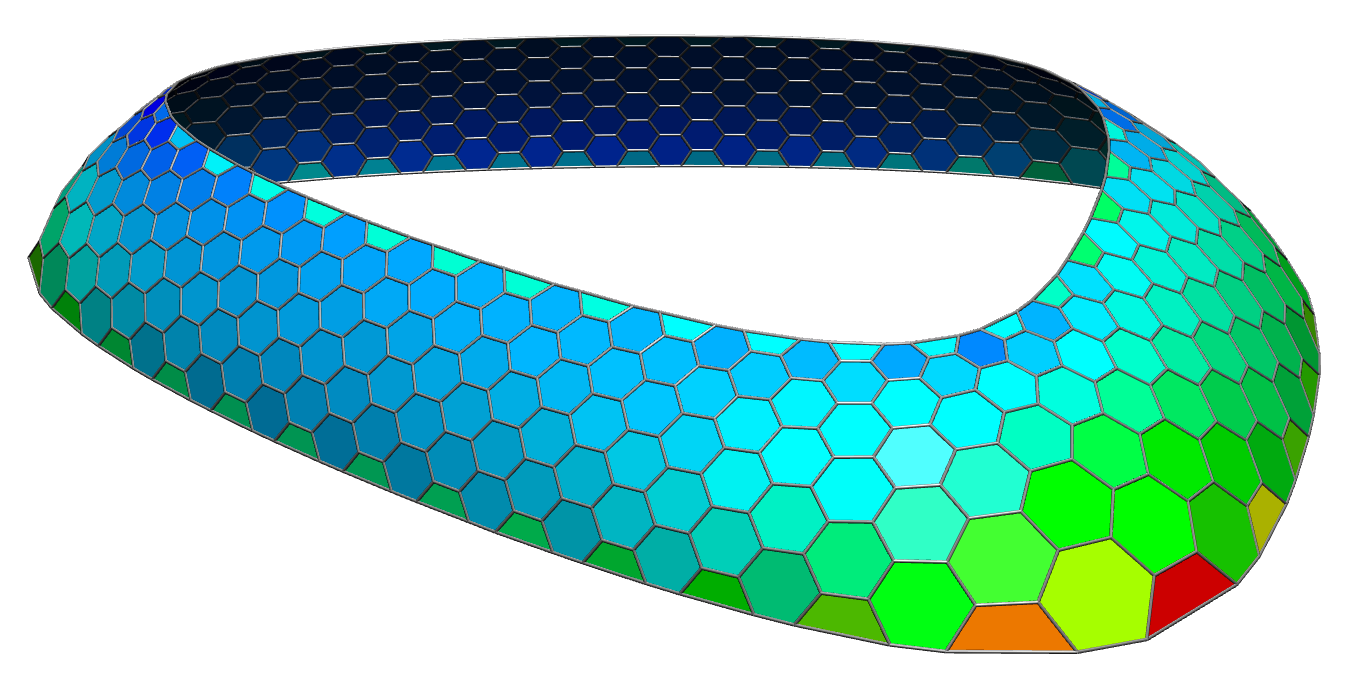
\includegraphics[width=5cm]{periodic/step08_surface.png}
            	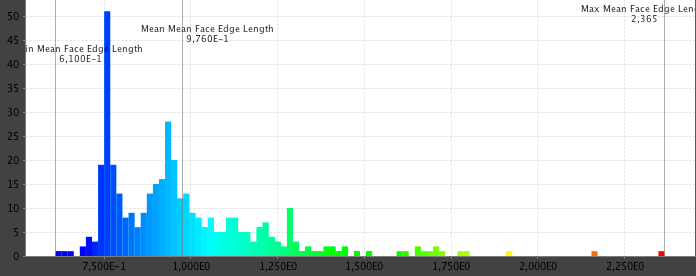
\includegraphics[width=5cm]{periodic/step08_histogram.png}		
            }
            \captionof{figure}{Measuring panel sizes and density with the [Halfedge Data Visualization] facility.}
\end{minipage}
\end{center}

\item[9] Equalize the edge lengths per face using the [Springs] Energy and [F-const] option. Use the [Floor] rounding method. Press [Update] to set target lengths per face.

\begin{center}
\begin{minipage}{0.9\linewidth}
            \centering
            \resizebox{\linewidth}{!}{
            	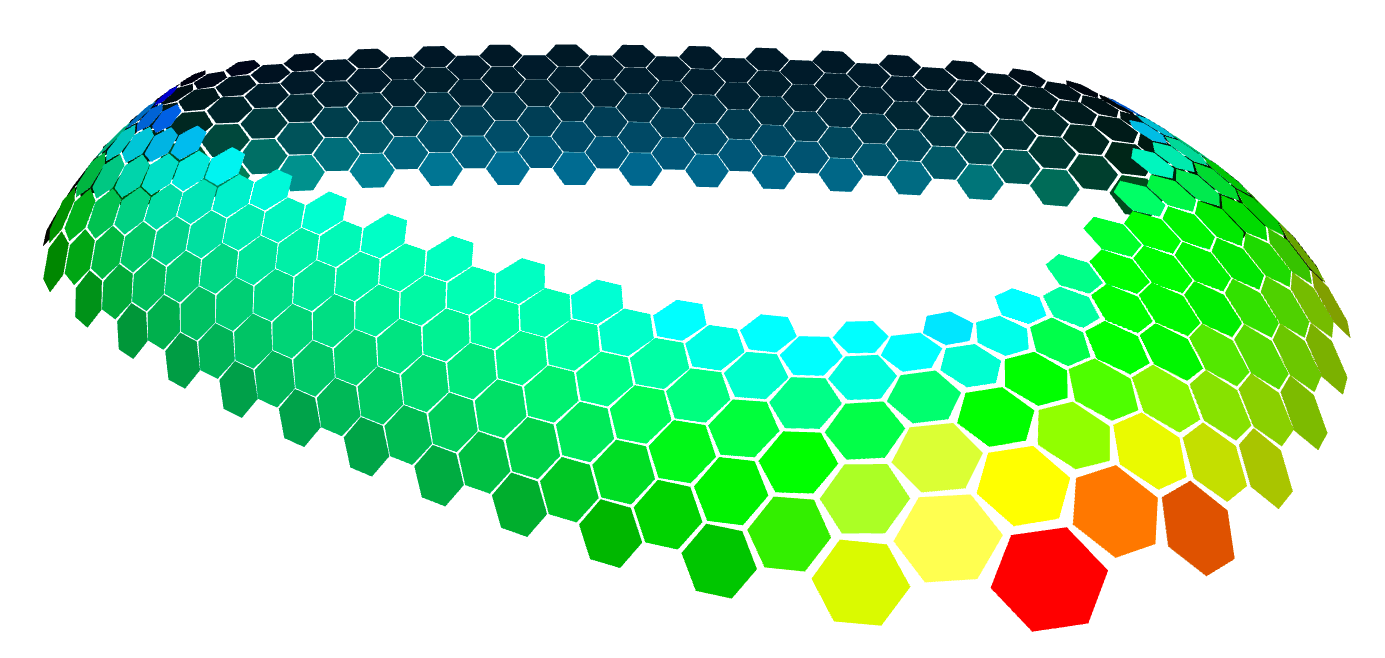
\includegraphics[width=13cm]{periodic/step09_surface.png}
            	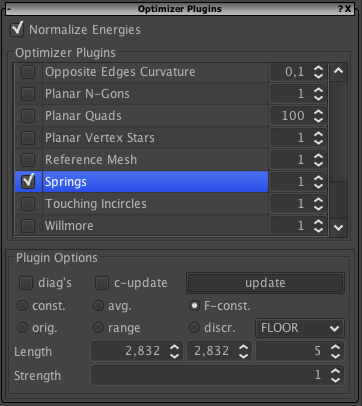
\includegraphics[width=5cm]{periodic/step09_fconst.png}
            }
            \captionof{figure}{Creating regular elements with the [Spring] energy.}
\end{minipage}
\end{center}
\item[10] From the histogram read off the smallest and largest edge lengths and transfer those into the [Springs] energy ui. Select the [discr.] option and the number of discrete steps. Optimize the surface to consist of a limited number of panel sizes.

\begin{center}
\begin{minipage}{0.9\linewidth}
            \centering
            \resizebox{\linewidth}{!}{
            	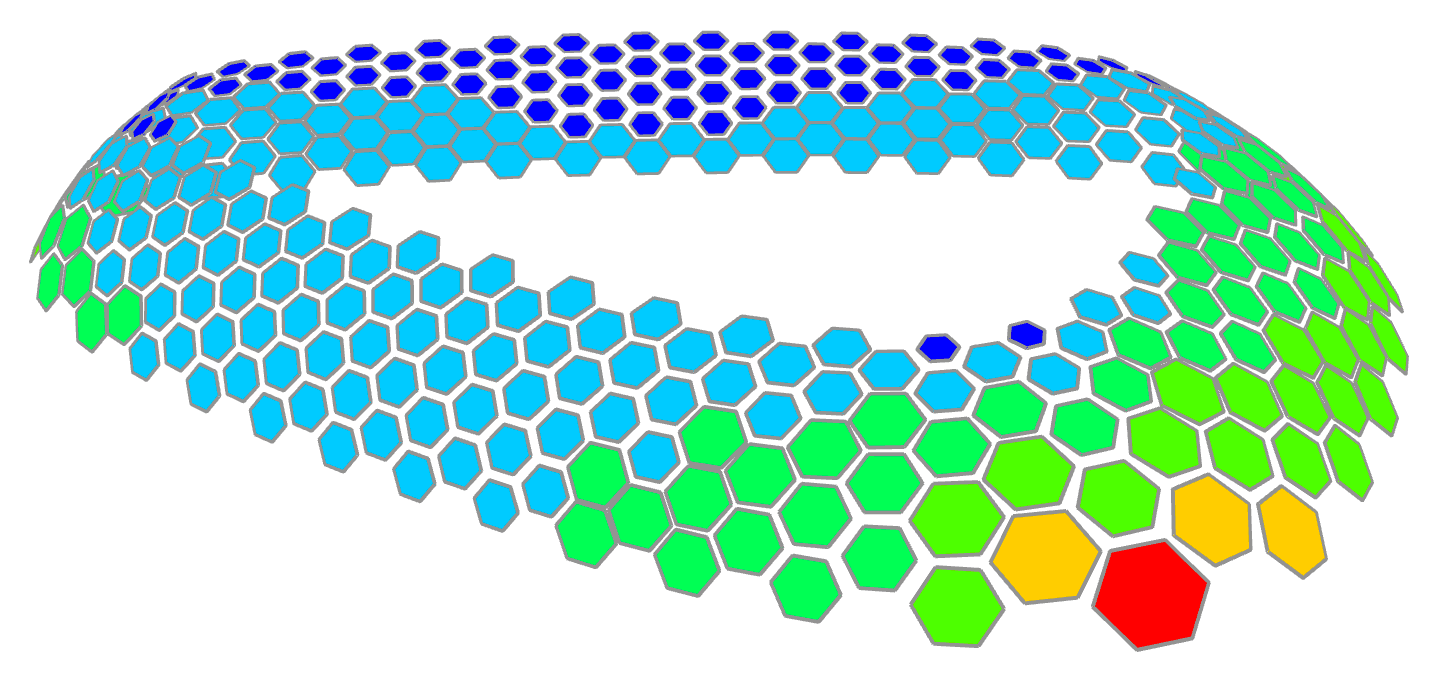
\includegraphics[width=13cm]{periodic/step11_surface1.png}
            	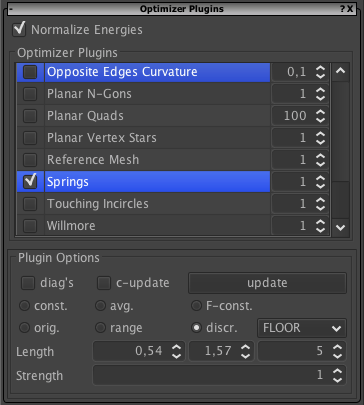
\includegraphics[width=5cm]{periodic/step10_springs.png}
            }
            \captionof{figure}{Optimization towards a discrete set of panel sizes.}
\end{minipage}
\end{center}            
\end{itemize}



\section{Quasiisothermic meshes with {\sc VaryLab}}
\label{sec:quasiisothermic_varylab}

\marginpar{\color{red}\footnotesize Split into two subsections: \\Parameterization and optimization \\for touching incircles.}

\begin{itemize}
\item[0] Load a genus $0$ surface with one boundary component.
\item[1] Calculate curvature direction estimates on interior vertices to find singularity locations and indices with the [Vector Field$\to$Curvature Vector Fields] command. Visualize directions using the [Halfedge Data Visualization] interface. The data is called, e.g., [Kmax Vec V] for maximum curvature direction with respect to the surface normal.
\item[2] Select singularity vertices and assign corresponding cone angles in the [Selected Nodes] panel of the [Discrete Conformal Parameterization] panel.
\item[3] Calculate curvature direction estimates on boundary edges of the surface, again using the [Vector Field$\to$Curvature Vector Fields] command. Check singularity indices with the [Check Gau{\ss}-Bonnet] button in the [Discrete Conformal Parameterization] panel. It prints the left side of the Gau{\ss}-Bonnet equation to the console. It should give $2\pi$ for a genus $0$ surface in this case.

\begin{center}
\begin{minipage}{0.9\linewidth}
            \centering
            \resizebox{\linewidth}{!}{
                \includegraphics[width=5cm]{quasiisothermic/step00.png}
                %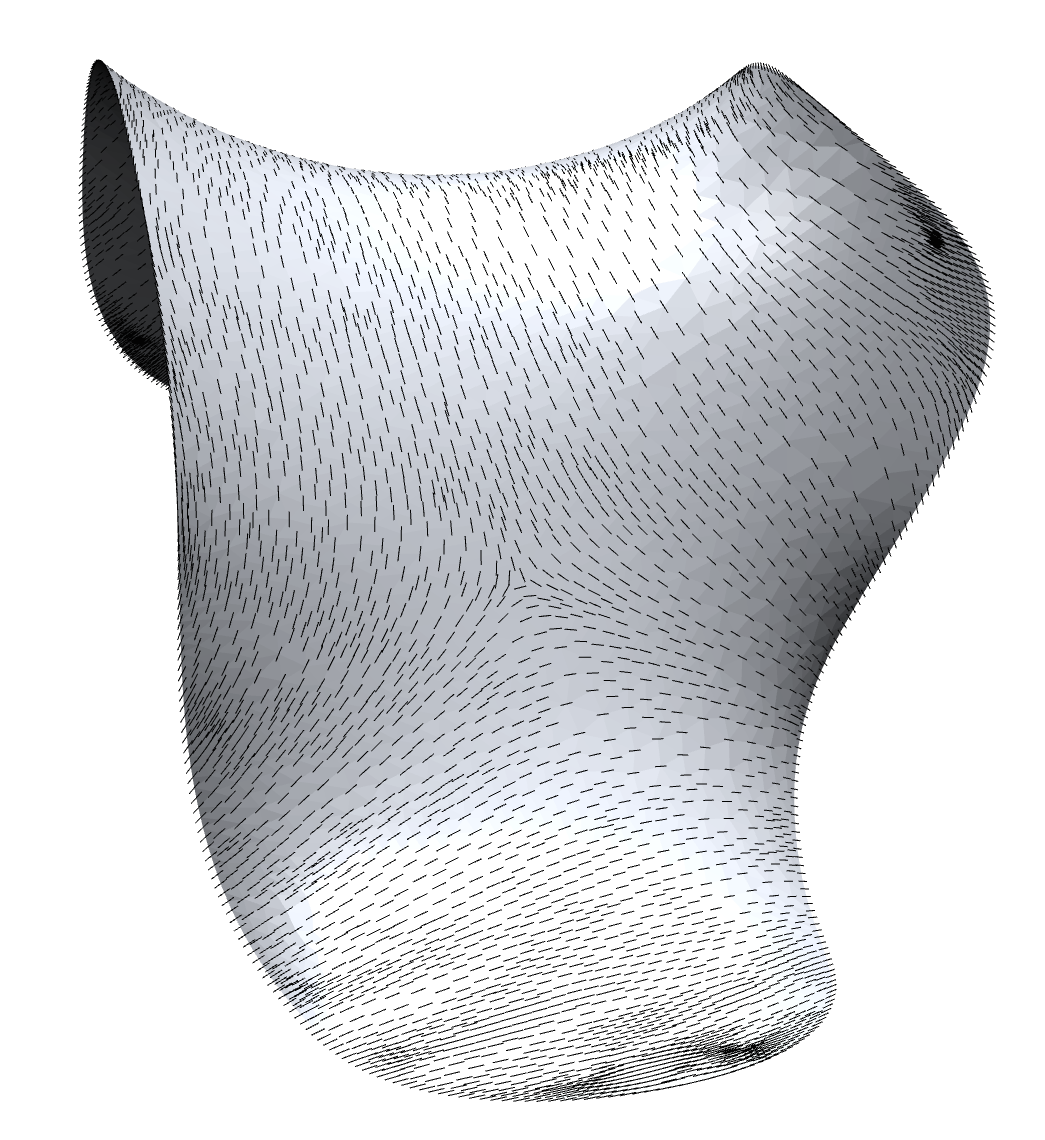
\includegraphics[width=5cm]{quasiisothermic/step01.png}
                \includegraphics[width=5cm]{quasiisothermic/step02_surface.png}
                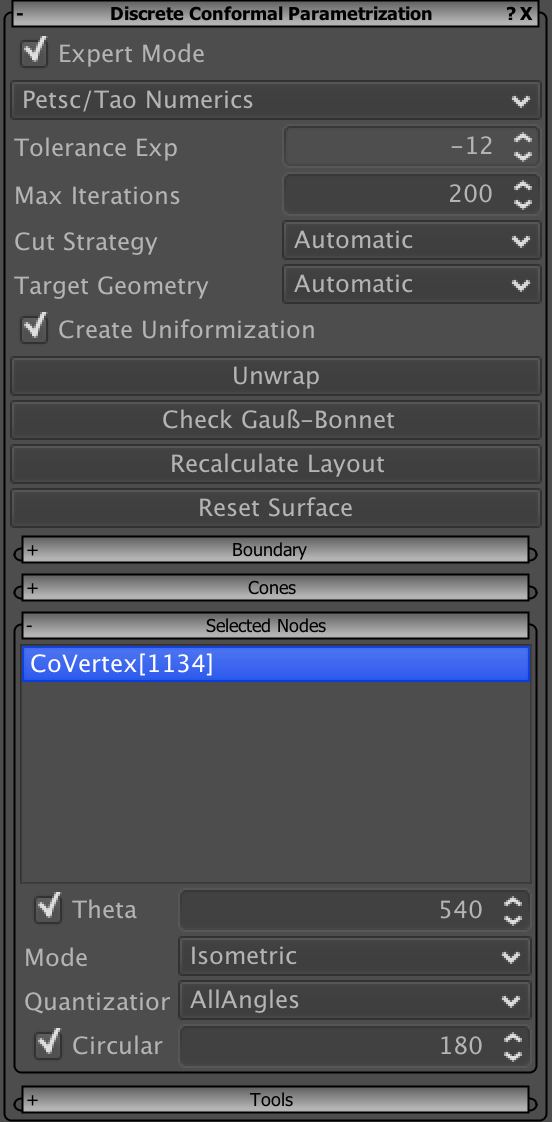
\includegraphics[width=2.6cm]{quasiisothermic/step02_ui.png}
                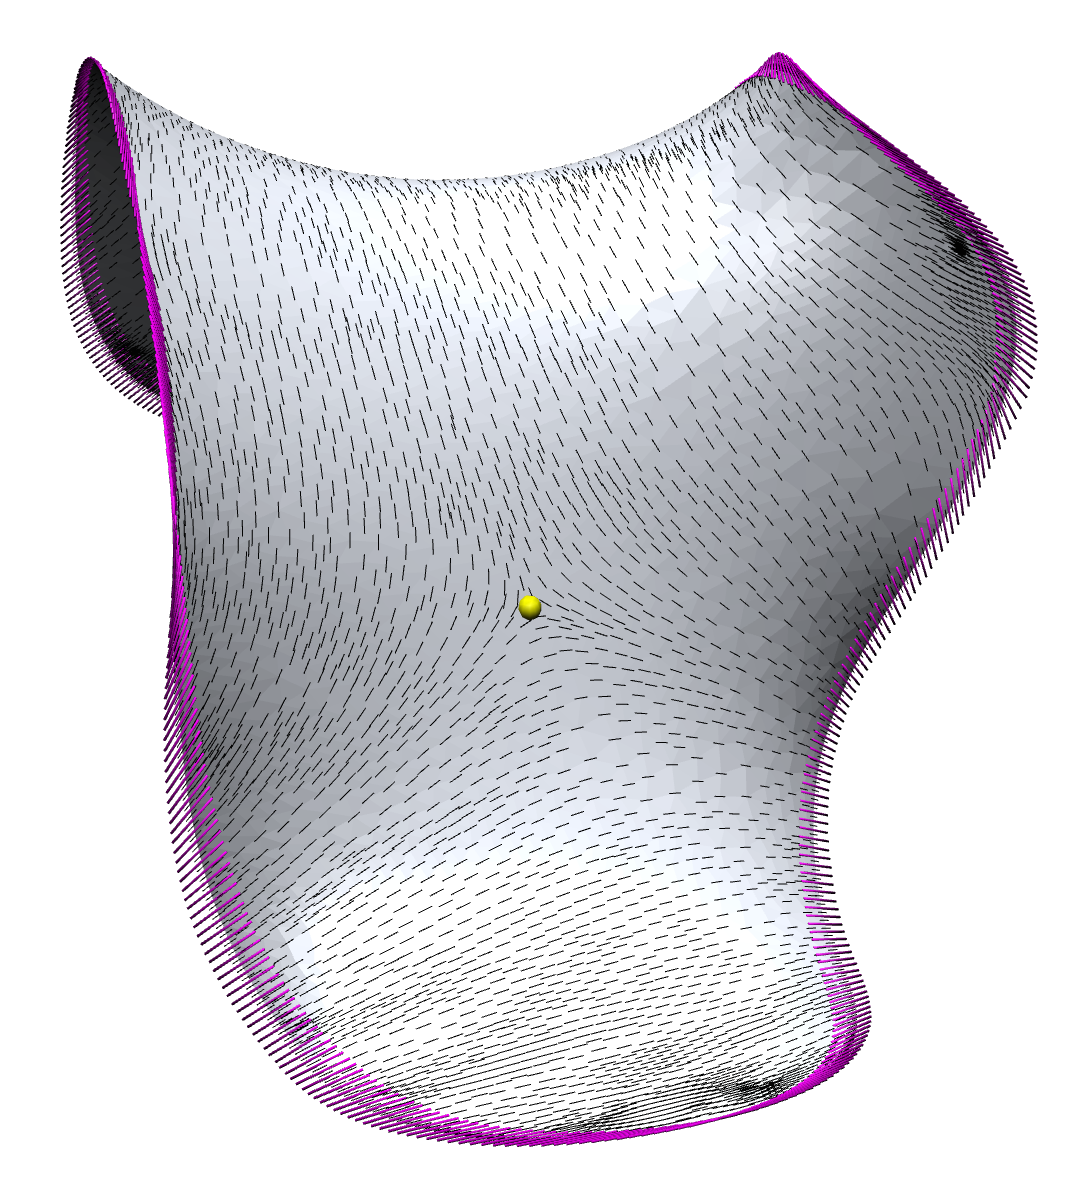
\includegraphics[width=5cm]{quasiisothermic/step03_surface.png}
            }
            \captionof{figure}{Inspecting the curvature direction field on the surface (middle) and specify boundary conditions (right, magenta) and singularities (right, yellow).}
\end{minipage}
\end{center}     
            
\item[4] Create a discrete conformal parameterization. Use [Conformal Curvature] as boundary mode. Select a quad texture to visualize the parameterization on the surface. Rotate the texture to match the prescribed boundary directions.
\item[5] Move the texture such that singularities lie either in the middle or at a corner of a quad of the texture. Use the [Texture Remeshing$\to$Transform Texture] command to transform the texture such that two selected vertices lie on $(0,0)$ and $(1,0)$ respectively. This method woks for one or two singularities. We do not implement methods to distort the mapping to match more that two singularities.

\begin{center}
\begin{minipage}{0.9\linewidth}
            \centering
            \resizebox{\linewidth}{!}{
                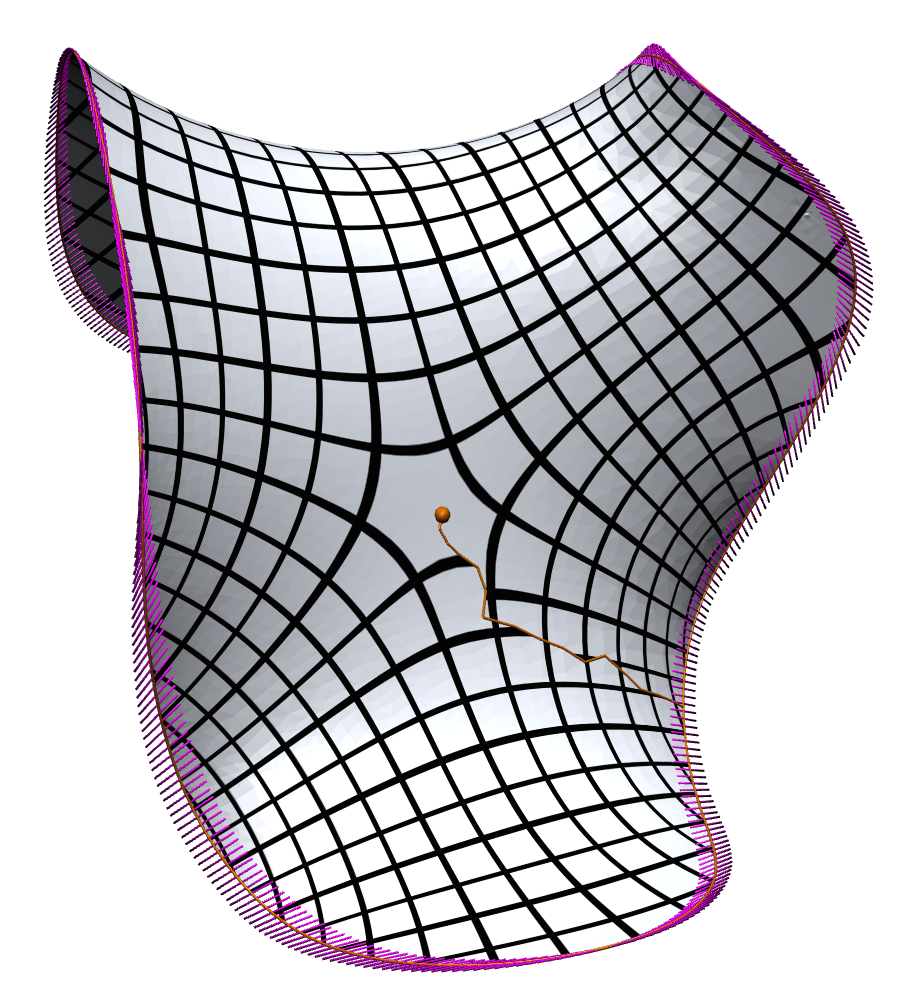
\includegraphics[width=5cm]{quasiisothermic/step04_surface.png}
                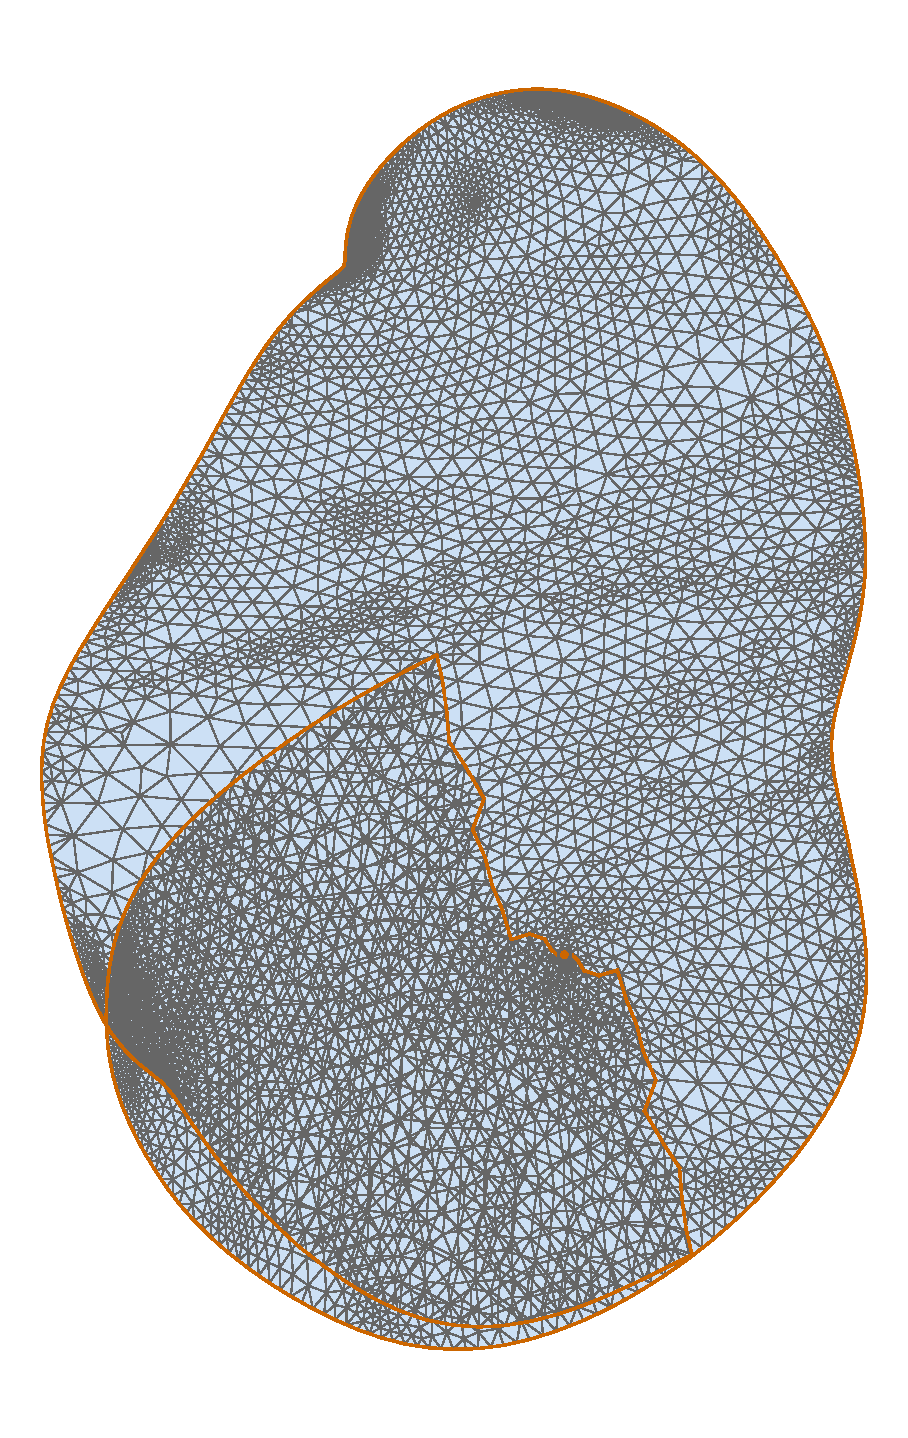
\includegraphics[width=4cm]{quasiisothermic/step04_map.pdf}
                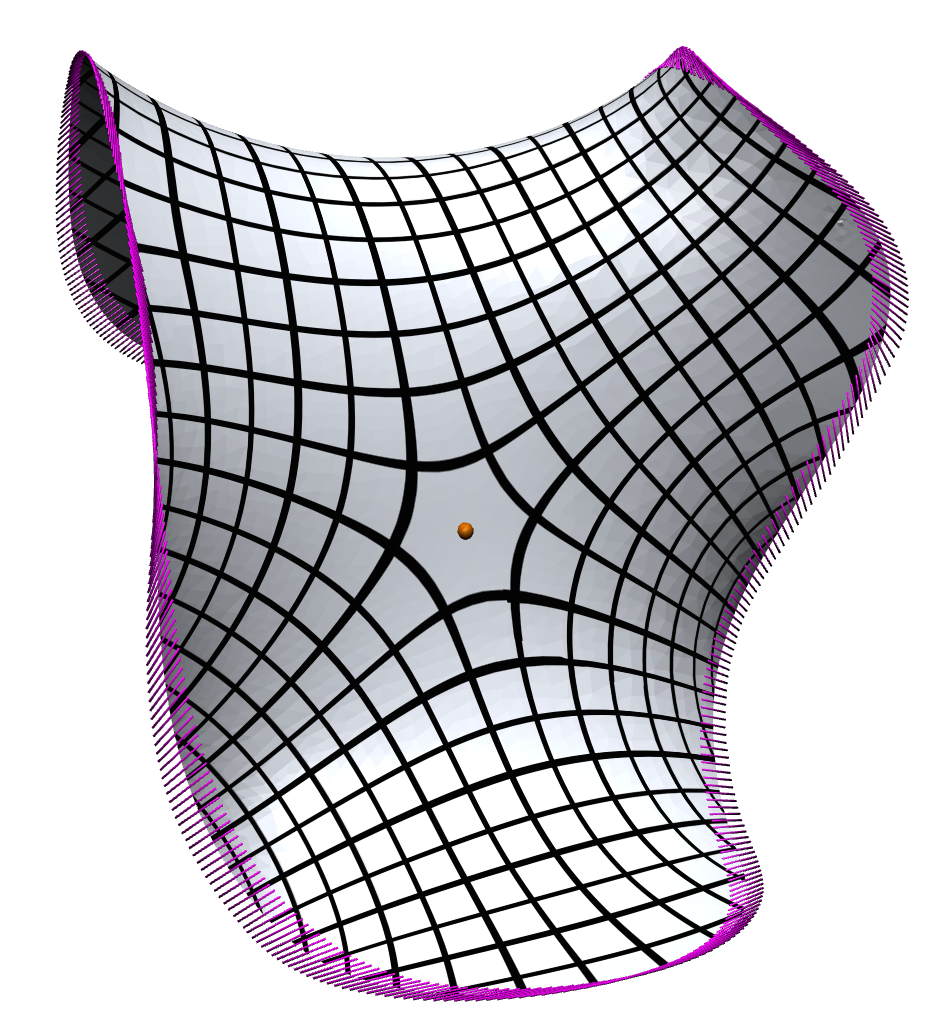
\includegraphics[width=5cm]{quasiisothermic/step05_surface.png}
            }
            \captionof{figure}{A quasiisothermic parameterization and its domain (left and middle). Move the singularity to a symmetry point of the pattern to close the parameter lines on the surface.}
\end{minipage}
\end{center}     
            
\item[6] Create a subdivision quad-mesh using the [Surface Remeshing] panel and the [Quads With Singularities] mode. This mode is available in the [Expert] mode of the panel. Press the [Lift/Flat] button to lift the subdivision to the surface.
\item[7] Use the [Texture Remeshing$\to$TextureGeometry] command to extract a quad mesh from the subdivision mesh. Disable the layer of the original mesh as we will continue to work with the quad-mesh.

\begin{center}
\begin{minipage}{0.9\linewidth}
            \centering
            \resizebox{\linewidth}{!}{
                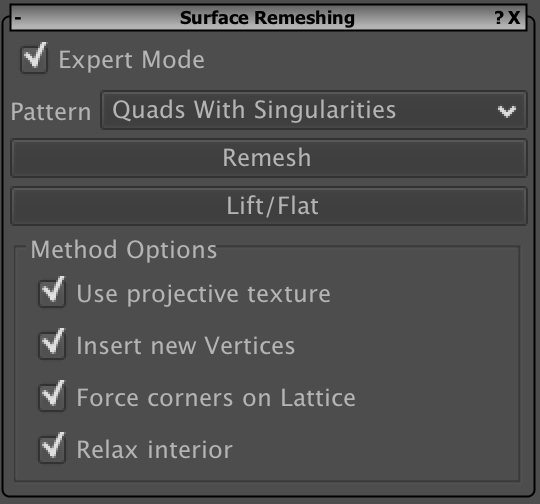
\includegraphics[width=4cm]{quasiisothermic/step06_ui.png}
                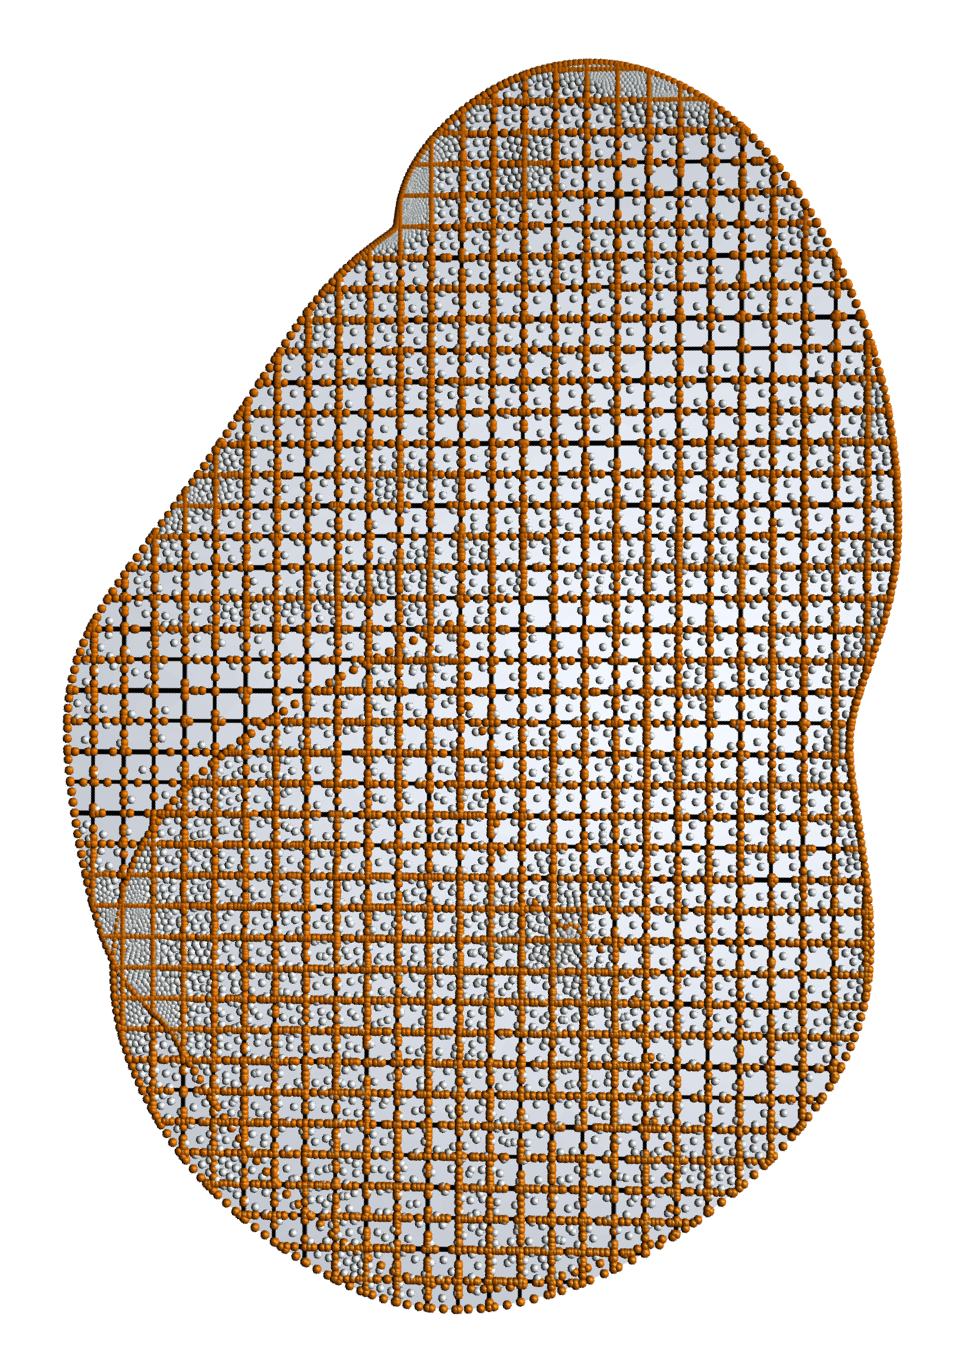
\includegraphics[width=4cm]{quasiisothermic/step06_flat_rotate.png}
                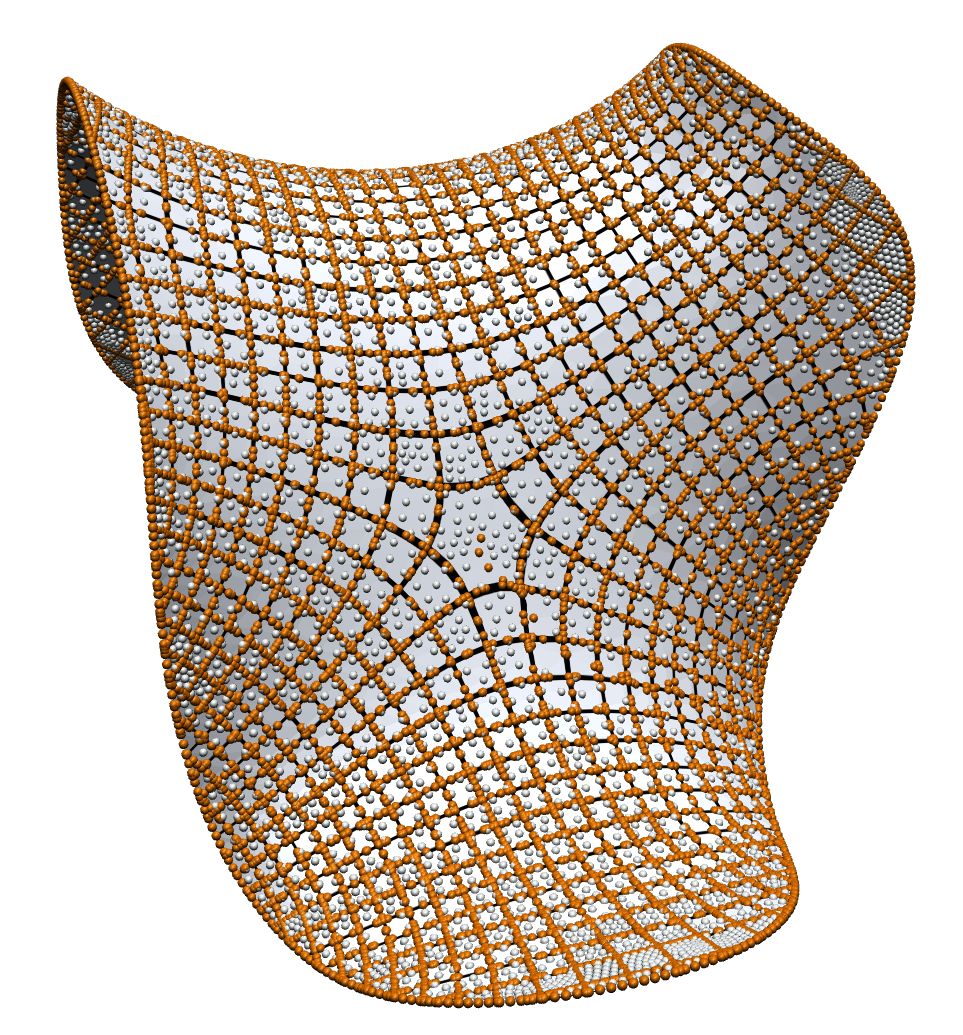
\includegraphics[width=5cm]{quasiisothermic/step06_surface.png}
                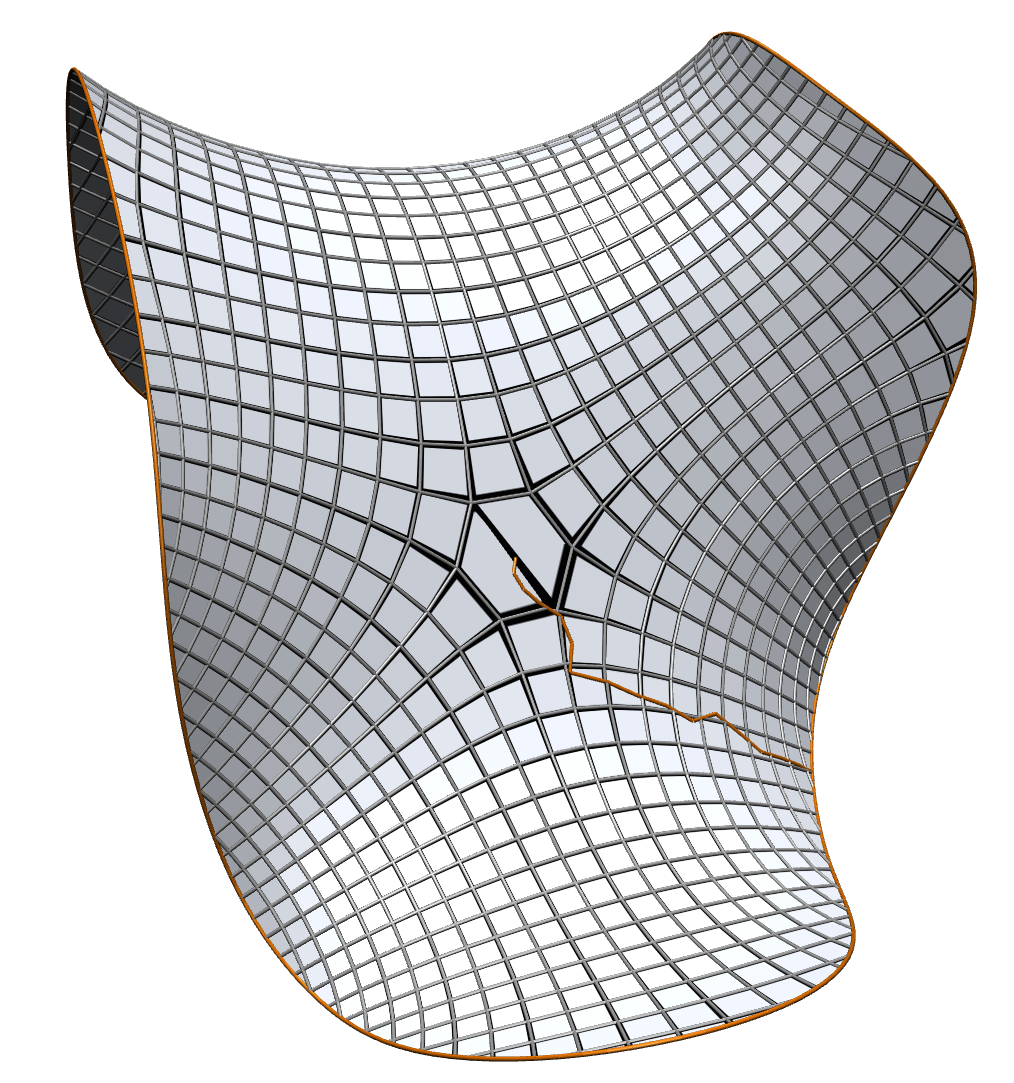
\includegraphics[width=5cm]{quasiisothermic/step07_surface.png}
            }
            \captionof{figure}{Three-step remeshing of the parameterized surface. Create a subdivided domain (second to left), lift this mesh to the surface (middle). Extract the new mesh from the subdivided (right).}
\end{minipage}
\end{center}                 
            
\item[8] Sew up the path from the boundary to the singularity using the [Topology$\to$ Stitch Cut Path] command. Select the two boundary vertices and a connected edge on the path.
\item[9] Remove extra vertices with the [Texture Remeshing$\to$Collapse 1,2-Valent Vertices] command.
\item[10] Clean up the mesh from extra edges and vertices with the [Selection$\to$Geodesic], [Edit$\to$Remove Edge And Fill], and [Texture Remeshing$\to$Collapse 1,2-Valent Vertices] command.

\begin{center}
\begin{minipage}{0.9\linewidth}
            \centering
            \resizebox{\linewidth}{!}{
                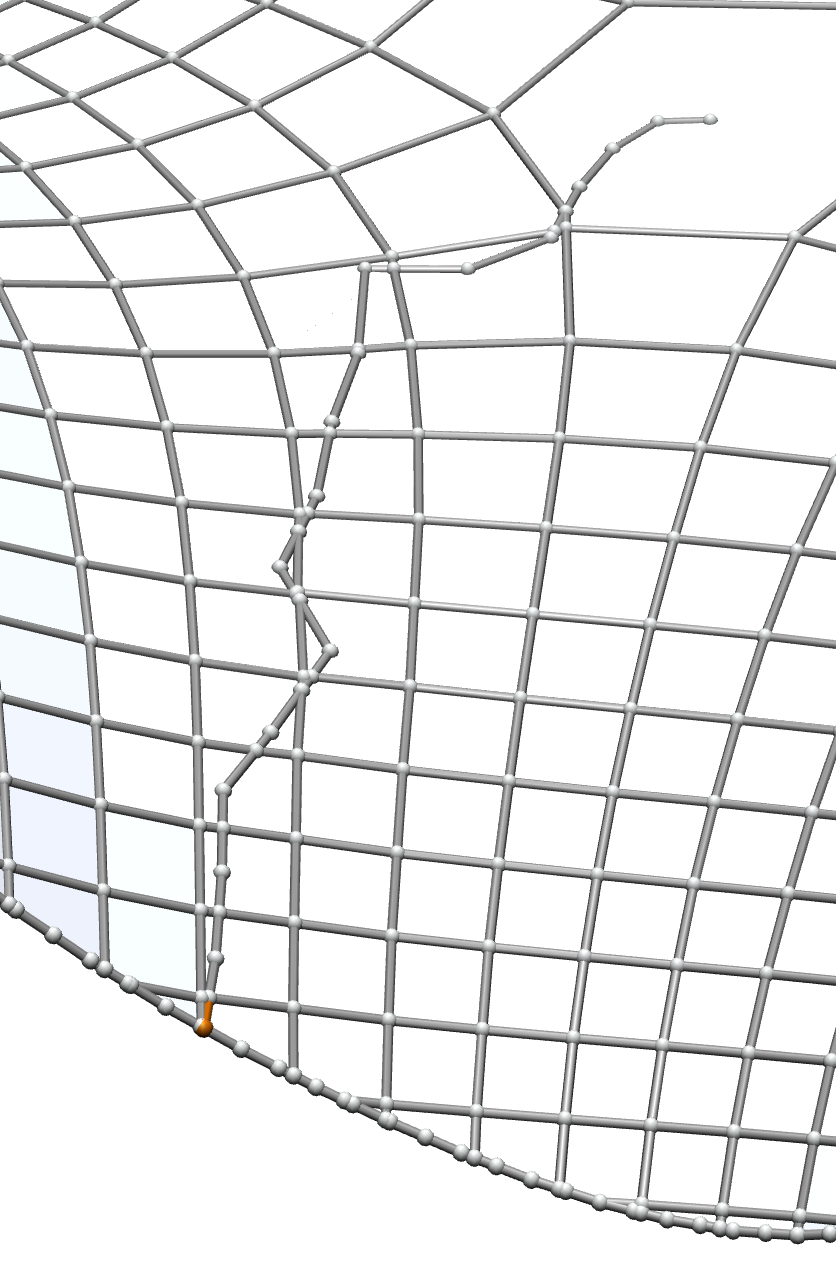
\includegraphics[width=3cm]{quasiisothermic/step08_selection.png}
                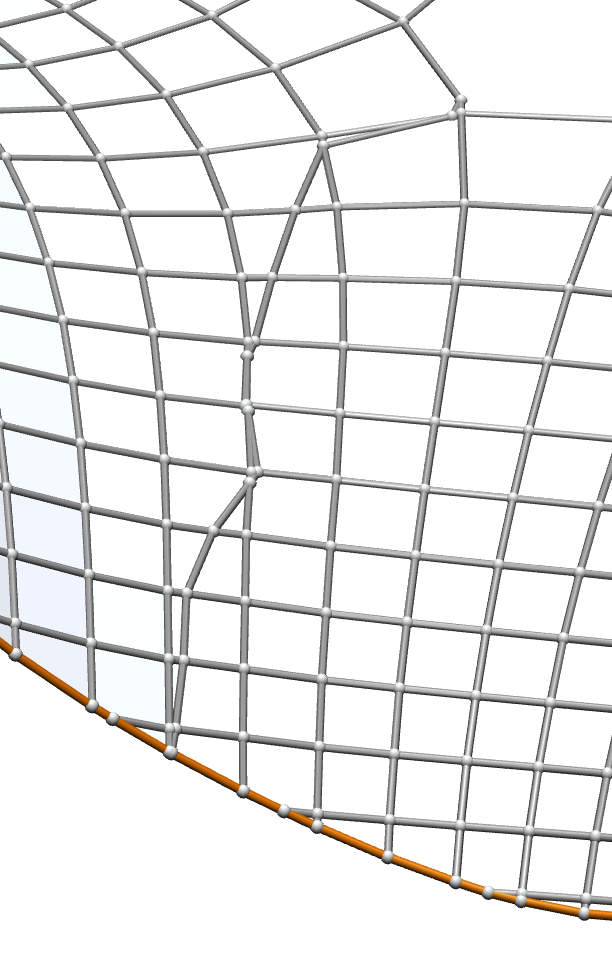
\includegraphics[width=3cm]{quasiisothermic/step09.png}
                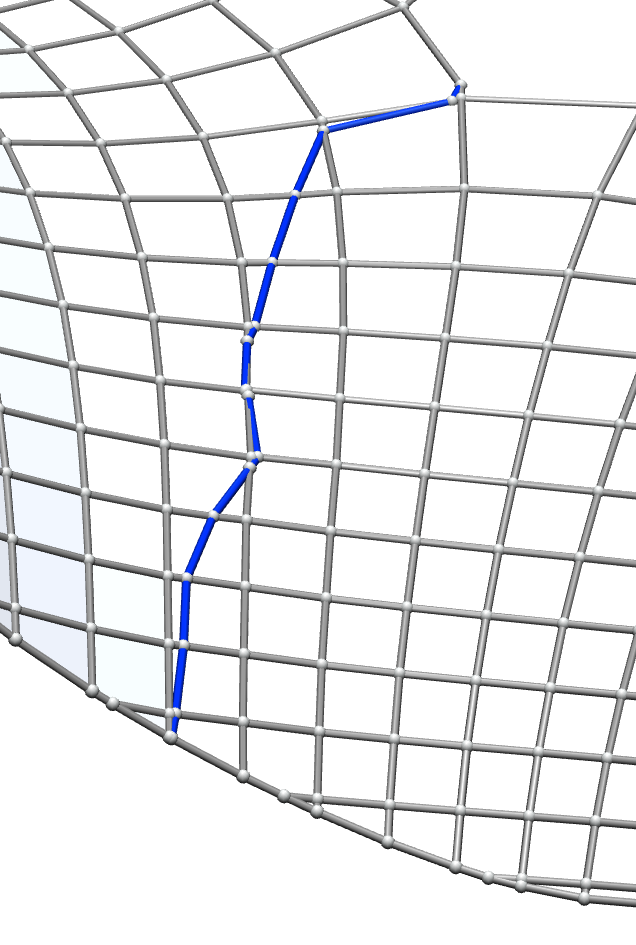
\includegraphics[width=3cm]{quasiisothermic/step10_selection.png}
                \includegraphics[width=5cm]{quasiisothermic/step10_surface.png}
            }
            \captionof{figure}{Removing the cut from a singularity to the boundary. Stitch the cut path by selecting the two vertices on the boundary and one adjacent edge on the path (left). Remove resulting vertices of valence $2$ (second to left). Select the path and remove extra edges.}
\end{minipage}
\end{center}    
            
\end{itemize}

\section{Gridshells with {\sc VaryLab}}
\label{sec:gridshells_varylab}

{\sc VaryLab} supports the creation of gridshell meshes, i.e., quadrilateral meshes with equal edge lengths. In this Section we describe how the results of Chapter~\ref{chp:gridshells} were created using the features of {\sc VaryLab}.

\begin{itemize}

\item[0] Design the target surface. The surface must be a topological disk. 
\item[1] Create an extended reference surface.

\begin{center}
\begin{minipage}{0.9\linewidth}
            \centering
            \resizebox{0.8\linewidth}{!}{
                \includegraphics[width=3cm]{gridshells/step0_target.png}
                \includegraphics[width=3cm]{gridshells/step1_extended.png}            
            }
            \captionof{figure}{The target shape design (left) and the extended surface used as reference surface (right).}
\end{minipage}
\end{center}    

\item[2] Discrete conformal parameterization using isometric boundary. 

\begin{center}
\begin{minipage}{0.9\linewidth}
            \centering
            \resizebox{0.8\linewidth}{!}{
                \includegraphics[width=3cm]{gridshells/step2_0degree.png}
                \includegraphics[width=3cm]{gridshells/step2_40degree.png}            
            }
            \captionof{figure}{Conformal parameterization with orthogonal parameter lines visualized with a quadrilateral texture (left). Parameter lines sheared by $40^\circ$ (right).}
\end{minipage}
\end{center}    

\item[3] Create a new quadrilateral mesh using the parameterization from step 2. You are free to shear the meshing pattern in the domain by an angle $\alpha$. From the [Surface Remeshing] panel choose the [Quads] mode and press [Remesh].

\begin{center}
\begin{minipage}{0.9\linewidth}
            \centering
            \resizebox{0.8\linewidth}{!}{
                \includegraphics[width=3cm]{gridshells/step3_0degree.png}
                \includegraphics[width=3cm]{gridshells/step3_40degree.png}            
            }
            \captionof{figure}{New quadrilateral meshes with orthogonal parameter lines (left) and parameter lines sheared by $40^\circ$ (right).}
\end{minipage}
\end{center}   

\item[4] Remove all boundary vertices and analyze the remaining edge lengths with node colors and histogram.

\begin{center}
\begin{minipage}{0.9\linewidth}
            \centering
            \resizebox{0.9\linewidth}{!}{
                \includegraphics[width=3cm]{gridshells/step4_surface.png}
                \includegraphics[width=4.5cm]{gridshells/step4_hist.png}            
            }
            \captionof{figure}{Edge length analysis. Target edge length should be below the mean edge length.}
\end{minipage}
\end{center}   

\item[5] Configure the optimization using the [Reference Surface] energy with the surface from step 1. Add the [Springs] energy with a constant edge length depending on the size of target surface. Finally add the [Opposite Edges Curvature] energy as a fairing term and to control the local curvature of curves.

\begin{center}
\begin{minipage}{0.9\linewidth}
            \centering
            \resizebox{\linewidth}{!}{
                \includegraphics[width=5cm]{gridshells/step5_ref.png}
                \includegraphics[width=5cm]{gridshells/step5_equal.png}            
                \includegraphics[width=7cm]{gridshells/step5_hist.png}                            
            }
            \captionof{figure}{Reference surface visualization (left). Optimized mesh (middle). Optimized histogram (right).}
\end{minipage}
\end{center}   

\end{itemize}

\subfilebibliography
\end{document}

%%% Local Variables:
%%% TeX-master: "Thesis.tex"
%%% End: